% ============================================================
%  Project Map and Intellectual Architecture
%  of the Flyxion Research Program
%  Working draft — lualatex
% ============================================================

\documentclass[12pt, twoside]{article}

% LuaLaTeX font setup — no fontenc/inputenc needed
\usepackage{fontspec}
\setmainfont{TeX Gyre Pagella}   % replaces tgpagella package
\usepackage{microtype}
\usepackage[margin=1.25in, headheight=14pt]{geometry}
\usepackage{setspace}
\usepackage{titlesec}
\usepackage{titletoc}
\usepackage{fancyhdr}
\usepackage{hyperref}
\usepackage{xcolor}
\usepackage{tikz}
\usetikzlibrary{arrows.meta, positioning, fit, backgrounds}
\usepackage{booktabs}
\usepackage{array}
\usepackage{longtable}
\usepackage{natbib}
\usepackage{enumitem}
\usepackage{abstract}
\usepackage{epigraph}

% ---- colour palette ----------------------------------------
\definecolor{rsvpblue}{HTML}{1B4F72}
\definecolor{cliogreen}{HTML}{1D6A39}
\definecolor{spherered}{HTML}{7B241C}
\definecolor{repairteal}{HTML}{117A65}
\definecolor{formalismgray}{HTML}{4A4A4A}
\definecolor{integgold}{HTML}{7D6608}
\definecolor{applviolet}{HTML}{4A235A}
\definecolor{lightbg}{HTML}{F7F9FA}

% ---- section formatting ------------------------------------
\titleformat{\section}{\large\bfseries}{\thesection.}{0.75em}{}
\titleformat{\subsection}{\normalsize\bfseries\itshape}{\thesubsection.}{0.75em}{}
\titleformat{\subsubsection}{\normalsize\itshape}{\thesubsubsection.}{0.75em}{}

% ---- headers -----------------------------------------------
\pagestyle{fancy}
\fancyhf{}
\fancyhead[LE]{\small\itshape Flyxion Research Program}
\fancyhead[RO]{\small\itshape Project Map}
\fancyfoot[C]{\thepage}
\renewcommand{\headrulewidth}{0.4pt}

% ---- spacing -----------------------------------------------
\setstretch{1.15}
\setlength{\parskip}{0.4em}
\setlength{\parindent}{1.5em}

% ---- hyperref ----------------------------------------------
\hypersetup{
  colorlinks=true,
  linkcolor=rsvpblue,
  citecolor=cliogreen,
  urlcolor=formalismgray,
  pdftitle={Project Map: Flyxion Research Program},
  pdfauthor={Flyxion}
}

% ---- framework entry command -------------------------------
% Two-command approach to stay within LaTeX's 9-argument limit.
% \frameworkhead{Name}{colour}{HistoricalOrigin}{KeyDependencies}{Purpose}
% \frameworkbody{Claim}{Objects}{Relations}{Papers}{Problems}
\newcommand{\frameworkhead}[5]{  \subsubsection{#1}
  \noindent\textcolor{#2}{\rule{\linewidth}{0.8pt}}
  \smallskip

  \noindent\textbf{Historical Origin.}\quad #3

  \noindent\textbf{Key Dependencies.}\quad #4

  \noindent\textbf{Purpose.}\quad #5
}
\newcommand{\frameworkbody}[5]{  \noindent\textbf{Central Claim.}\quad #1

  \noindent\textbf{Core Objects.}\quad #2

  \noindent\textbf{Relationships to Other Frameworks.}\quad #3

  \noindent\textbf{Major Works.}\quad #4

  \noindent\textbf{Open Problems.}\quad #5
  \medskip
}
% Compatibility wrapper: \framework{Name}{col}{Orig}{Dep}{Purp}{Claim}{Obj}{Rel}{Works}
% splits into head (args 1-5) + body (args 6-9 + final brace group)
% Because we need 10 logical args, we use a relay via two calls.
% Direct usage: call \frameworkhead then \frameworkbody in sequence.


% ============================================================
\begin{document}

% ---- title page --------------------------------------------
\begin{titlepage}
\centering
\vspace*{2cm}
{\Huge\bfseries Project Map and Intellectual Architecture}\\[0.6em]
{\Large\bfseries of the Flyxion Research Program}\\[2em]
{\large Working Draft}\\[0.4em]
{\normalsize\itshape The Admissibility Program: From Practice and Intuition\\
to Cosmology, Cognition, Computation, and Civilisation}\\[3em]
{\large Flyxion}\\[0.5em]
{\normalsize Independent Researcher\\[0.2em]
\today}
\vfill
\begin{abstract}
\noindent
This document maps the intellectual architecture of the Flyxion research
program as it stands at the time of writing. The program spans cosmological
field theory, formal ontology, cognitive architecture, memory theory,
process-native computation, and civilisational geometry. Despite their
apparent diversity, these projects share a common organising principle: the
claim that every domain of inquiry is fundamentally concerned with the
maintenance, loss, restoration, and navigation of \emph{admissible
transformations}. This organising principle is called the Admissibility
Program. The document is organised in three parts. Part~I traces the
origins of the program from direct practical engagement with construction,
repair, and physical restoration through the convergence of core intuitions
into formal frameworks. Part~II presents the current architecture as a
five-layer structure: practice and embodied knowledge, core intuitions,
theoretical frameworks, formalization programs, and domain applications.
Part~III surveys the major open problems whose resolution would most
significantly advance the program. An appendix provides a
framework-by-framework reference guide following a common template.
\end{abstract}
\end{titlepage}

% ---- table of contents -------------------------------------
\tableofcontents
\newpage

% ============================================================
\part*{Part I\quad Origins and Convergence}
\addcontentsline{toc}{part}{Part I: Origins and Convergence}

\section{Practice as the Ground Floor}

The oldest and most underacknowledged layer of the Flyxion research program
is not theoretical. It is practical. Over many years, direct engagement with
construction, electrical work, plumbing, property rehabilitation, and
custom home building produced a body of embodied knowledge about systems that
cannot be rebuilt from scratch and must instead be restored while maintaining
continuity of function.

This matters for the intellectual history of the program because the
distinctive character of the theoretical work is difficult to explain without
it. The decision to treat repair as more fundamental than construction does
not feel like an abstraction invented in isolation. It reads as a
formalization of intuitions accumulated from repeatedly encountering physical
systems in which replacement is not an option and continuity must be actively
maintained despite degradation. Similarly, the insistence on reachability
over location, on process over object, and on accessibility over distance all
have natural analogues in the practical experience of working within
constraint-laden systems where the question is never \emph{what is the ideal
structure?} but always \emph{what transformations are actually available from
here?}

The connection between practice and theory is not merely biographical. It has
structural consequences for the program. A theoretical framework that began
from armchair reflection about physical systems might have taken objects,
positions, and states as its primitive concepts. A framework that grew from
sustained practical engagement with repair, restoration, and constrained
transformation is more likely to take processes, trajectories, and
accessibility as its primitives — because those are the concepts that do
actual work in the practice.

This suggests that the correct genealogy of the Admissibility Program is
best understood not as a flat stack but as a geological stratigraphy — each
layer deposited over the one below, with the deepest layers conditioning
everything above them.

\begin{center}
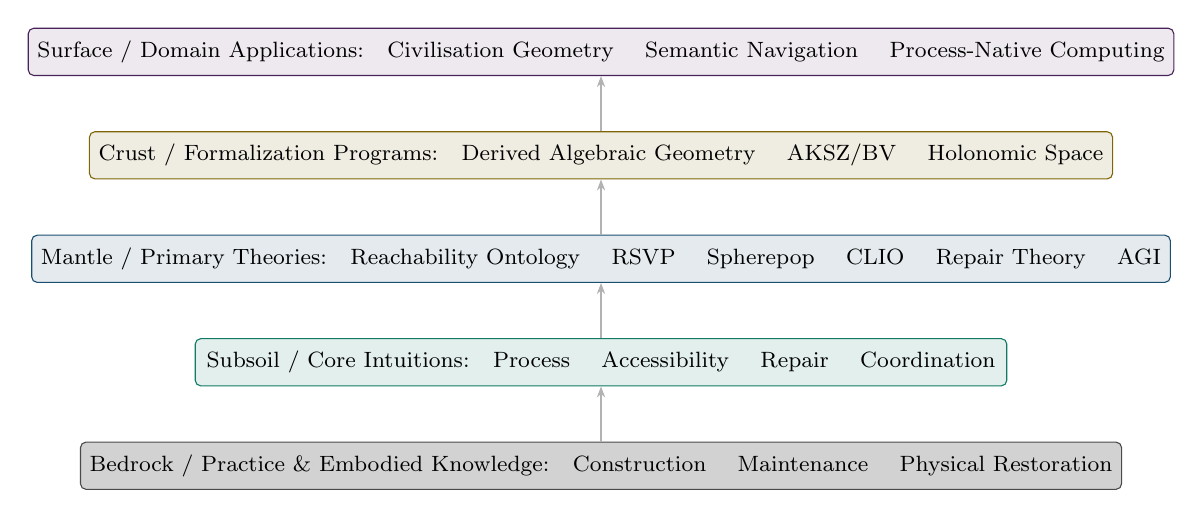
\begin{tikzpicture}[
  node distance=0.7cm,
  every node/.style={font=\footnotesize, align=center},
  layer/.style={draw=formalismgray, rounded corners=2pt,
                fill=lightbg, minimum width=0.85\textwidth, minimum height=0.6cm},
  bedrock/.style={layer, fill=formalismgray!25, draw=formalismgray},
  subsoil/.style={layer, fill=repairteal!12, draw=repairteal},
  mantle/.style={layer, fill=rsvpblue!12, draw=rsvpblue},
  crust/.style={layer, fill=integgold!12, draw=integgold},
  surface/.style={layer, fill=applviolet!10, draw=applviolet},
  lbl/.style={font=\footnotesize\bfseries, anchor=east},
  arr/.style={-{Stealth[length=4pt]}, gray!60}
]
\node[surface]  (S) {Surface / Domain Applications:\quad Civilisation Geometry \quad Semantic Navigation \quad Process-Native Computing};
\node[crust, below=of S]   (C) {Crust / Formalization Programs:\quad Derived Algebraic Geometry \quad AKSZ/BV \quad Holonomic Space};
\node[mantle, below=of C]  (M) {Mantle / Primary Theories:\quad Reachability Ontology \quad RSVP \quad Spherepop \quad CLIO \quad Repair Theory \quad AGI};
\node[subsoil, below=of M] (I) {Subsoil / Core Intuitions:\quad Process \quad Accessibility \quad Repair \quad Coordination};
\node[bedrock, below=of I] (B) {Bedrock / Practice \& Embodied Knowledge:\quad Construction \quad Maintenance \quad Physical Restoration};
\draw[arr] (B) -- (I);
\draw[arr] (I) -- (M);
\draw[arr] (M) -- (C);
\draw[arr] (C) -- (S);
\end{tikzpicture}
\end{center}

\medskip

This layering also resolves an apparent paradox in the corpus: why a body of
work ostensibly concerned with cosmology, cognition, and computation keeps
returning to the vocabulary of maintenance, preservation, and repair. The
vocabulary is not metaphorical. It is originary.

\section{The Phase Before the Map}

\epigraph{\itshape Reality is Reachability. Keep the branches open.}{}

Every large research program passes through a phase in which one framework
acts as a universal attractor. Questions from unrelated domains get drawn
toward it, reformulated in its vocabulary, and answered by extending its
machinery. During the earliest documented phase of the Flyxion program, that
attractor was the Relativistic Scalar-Vector Plenum, or RSVP.

During this period, RSVP was not merely one theory among several. It was the
lens through which gravity, entropy, structure formation, cosmological
evolution, consciousness, and institutional behaviour were all being
re-examined simultaneously. The intellectual portfolio of that period
reflects this: the formalization program pursued derived algebraic geometry,
AKSZ and Batalin-Vilkovisky quantization, shifted symplectic structures, and
derived sigma models, all in the service of putting RSVP on rigorous
mathematical footing. The RSVP Field Simulator evolved from earlier
continental-drift and biomass simulations into a genuine field-theoretic
environment. A thread extending RSVP into consciousness dynamics asked what
admissibility-field concepts implied about cognition and subjective
experience.

That early period raised the question: \emph{If RSVP is correct, what
mathematical structures are required to express it rigorously?}

The question was productive. But a second, deeper question gradually emerged
alongside it, one that was not narrowly about RSVP at all: \emph{What is the
architecture of admissibility across physics, cognition, memory, computation,
repair, and civilisation?}

The shift from the first question to the second marks the transition that
this document is intended to record. The first question is largely a physics
question and asks for equations. The second is a systems question and asks
for relationships among frameworks. The transition did not abandon the
earlier work; RSVP formalization remains an open program. But the center of
gravity migrated from a single theory to a broader set of interlocking
frameworks organised around a common underlying concept.

\section{Four Recurring Intuitions}

Surveying the corpus, the intellectual history is better described as a
convergence of recurring intuitions than as a strict genealogy of derived
results. Several of the major frameworks appear to have crystallised
independently before their mutual dependencies became visible.

The first intuition is process over object. Across cosmology, cognition,
language, and computation, the early papers consistently resist the
assumption that the fundamental constituents of a domain are discrete
objects. Trajectories, flows, relaxations, collapses, and activations appear
as more primitive than the stable entities they produce.

The second intuition is accessibility over location. Spatial and semantic
proximity are repeatedly set aside in favour of questions about what states a
system can reach. Metric distance is treated as derived; reachability is
treated as more fundamental. This intuition appears in cosmological work on
admissibility regions, in memory theory as retrieval thresholds, in
institutional analysis as fiscal reachability, and in search theory as
preference fields on semantic manifolds.

The third intuition is persistence over construction. Stable structures are
more often explained as the outcome of active maintenance than as the
consequence of initial assembly. Repair, restoration, and the preservation of
admissible states are repeatedly invoked to explain why structures endure
rather than how they were first built.

The fourth intuition is coordination over centralised control. Distributed
systems across brains, institutions, antennas, and ecosystems are explained
by reference to how components synchronise their local constraints rather than
how a global controller directs them.

Each major framework in the program can be understood as a rigorous
development of one or more of these four intuitions applied to a particular
domain. The Reachability Ontology articulates them philosophically. RSVP
formalises the first and second in a field-theoretic language. Spherepop
develops the first in an event-theoretic language. Repair Theory develops the
third as an independent claim. Coordination Geometry develops the fourth
empirically and mathematically.

\section{Precursor Works and Recovered Threads}

Comparison across several project inventories from different periods reveals
a number of works that later summaries omitted but which deserve recognition
as early statements of the broader program.

\emph{Persistent Anomalies and the Geometry of Ontology Revision} now
appears to be one of the earliest explicit statements of the admissibility
perspective. Its framework for distinguishing minor errors from fundamental
structural failures in data models through topological obstructions and
repair theory anticipates both Repair Theory and CLIO in significant ways.
It also establishes the vocabulary of obstruction that later appears in the
sheaf-theoretic strand of TARTAN. This monograph should be treated as a
precursor text rather than a peripheral application.

\emph{Holonomic Space: Admissibility and Reconstruction} represents a
significant formalization effort that sits between RSVP and the
derived-geometry program. Its focus on variational dynamics, sheaf theory,
and observational programs for modelling cosmology and measurement through
local recursive persistence gives it a character distinct from both the
physical RSVP papers and the purely mathematical formalization work. It
deserves recognition as an independent formalization program alongside
derived algebraic geometry and AKSZ/BV quantization.

\emph{The Geometry of Rewiring: Ecological Networks, Admissible Trajectories,
and the Conservation of Transformability} was one of the earliest successful
applications of admissibility thinking outside cosmology and cognition. Its
reinterpretation of ecological resilience as the preservation of navigable
future paths demonstrates that the admissibility framework was already capable
of domain transfer at an early stage.

\emph{The Stone Piano Hypothesis}, which investigates whether 176,500-year-old
Neanderthal structures in Bruniquel Cave functioned as intentional
lithophones, does not fit neatly into the main dependency graph. It is a
domain investigation in archaeological acoustics. Its presence in the corpus
is a reminder that the program has always maintained peripheral research
interests that are intellectually motivated without being theoretically
derivative.

\emph{Calculus as the Geometry of Relationship and Controlled Change} belongs
to the pedagogical layer. Its reframing of calculus as a geometric language
for transformation expresses the same core intuitions as the larger program
and may function as one of its most accessible entry points.

One thread deserves specific attention because its transformation is
illustrative of the broader pattern. RSVP Consciousness Dynamics began as a
direct extension of the scalar-vector plenum framework into the theory of
cognition. Thermodynamic gradients, information flows, and admissibility
measures were being used to construct a theory of subjective experience
grounded in field dynamics.

That program did not produce a standalone pillar in the current architecture.
Instead, its concerns appear to have been distributed across several later
frameworks. Questions about how cognitive systems project and compress their
experienced landscape migrated into CLIO. Questions about the formation,
persistence, and collapse of mental structures migrated into Spherepop.
Questions about memory retrieval and reactivation migrated into
Preservation/Ecphory. Questions about how neural systems coordinate migrated
into Coordination Geometry. The integration of these answers into a
full cognitive architecture became the project now known as HYDRA.

The lesson the transition illustrates is one that recurs throughout the
program's history. What appears initially as an extension of a single
framework often turns out to be a question requiring coordination across
multiple frameworks. The eventual response to that insight was structural: the
development of integrative frameworks capable of drawing simultaneously on
primary theories.

\section{The Wider Speculative Corpus}

A project inventory from April 2025 reveals a substantially wider range of
work than the dependency graph of the core Admissibility Program suggests.
That inventory lists approximately one hundred active projects spanning
cognitive systems, speculative physics, environmental engineering,
civilisation-scale simulation, philosophy of language, hardware prototypes,
governance theory, music, and cultural artefacts. Most of these do not appear
in the main architecture and are not derived from the primary frameworks in
any straightforward sense.

This requires an honest accounting of what the project map is and is not
doing. The map presented in Part~II describes the \emph{theoretical core}:
the frameworks that repeatedly generate new concepts, formal structures, and
research questions recurrent across the corpus. That core is real, and the
dependency relationships within it are genuine. But it accounts for perhaps a
third of the intellectual output by volume. The remaining work consists of
speculative projects that may be loosely inspired by the core intuitions
without being formally derived from them.

Several examples illustrate the range. Within cognitive systems, projects
such as Aspect Relegation Theory, the Inforganic Codex, the Trodden Path
Mind, Semantic Ladle Theory, the Substrate Independent Thinking Hypothesis,
and Geometric Bayesianism with Sparse Heuristics constitute substantial
speculative frameworks in their own right. Their relationship to the
Admissibility Program is one of family resemblance rather than derivation:
they share the program's preference for process, trajectory, and constraint,
but have not been formally integrated into the dependency graph.

Within speculative physics, projects including Crystal Plenum Theory, the 5D
Ising Synchronization Model, the Neutrino Fossil Registry, and
Universe-as-Sponge Cosmology extend or contest the RSVP framework from
various directions. Lamphron and Lamphrodyne States, which name specific
relaxation phenomena within RSVP, are effectively internal subdivisions of
the primary theory rather than independent alternatives.

Within environmental and terraforming systems, the Cyclex Climate
Stabilisation Architecture, Volsorial Pediments, Gravitational Batteries, and
Orthodromic Rivers constitute a body of speculative infrastructure engineering
whose central concern — what transformations are admissible for a
constrained planetary environment under climate pressure — is structurally
continuous with the core program even though the technical content is
primarily engineering rather than formal theory.

Within hardware prototypes and cultural artefacts, work such as the
Ontological Dishwasher, Mechatronic Diapers, and Recursive Cloakproof Chain
Generator reads as speculative design objects, satirical interventions, or
thought experiments in material form. They belong to what might be called the
\emph{mythopoetic layer}: work that enacts the program's commitments in
unexpected registers rather than formalising them.

The correct response to this breadth is not to expand the dependency graph
until it contains everything. That would destroy the graph's utility as a
map. Instead, the architecture should be understood as having a dense
theoretical core surrounded by a larger halo of speculative, satirical,
pedagogical, and mythopoetic work that maintains a family relationship with
the core without being formally derivable from it. The core provides the
vocabulary and the commitments; the halo explores, tests, parodies, and
extends them in registers that formal theory cannot reach.

% ============================================================
\part*{Part II\quad The Current Architecture}
\addcontentsline{toc}{part}{Part II: The Current Architecture}

\section{Overview: A Five-Layer Architecture}

The current architecture is best described as a five-layer dependency
structure in which each layer draws on the one below it while generating
new objects, questions, and methods that feed upward.

The first layer is practice: the embodied knowledge of construction, repair,
restoration, and constrained physical transformation that generated the
program's foundational intuitions.

The second layer is the four core intuitions that were extracted from that
practice and that run consistently through all subsequent theoretical work:
process over object, accessibility over location, repair over construction,
and continuity over replacement.

The third layer is the theoretical frameworks proper. Within this layer the
architecture is not a tree but a dependency graph, since several frameworks
are junction nodes drawing on more than one upstream theory. The foundational
ontology sits at the base of this layer; the primary theories develop it;
the secondary formalisms extend and connect the primary theories; and the
integrative frameworks synthesise multiple inputs simultaneously.

The fourth layer is the formalization programs: mathematical and
computational efforts to express the theoretical frameworks with greater
rigour. These include the derived algebraic geometry formalization of RSVP,
the AKSZ/BV quantization program, the Holonomic Space program, the RSVP
Field Simulator, and related tools.

The fifth layer is domain applications: instantiations of the theoretical
frameworks in specific empirical and practical domains including cognition,
search, computing, civilisation, ecology, and cosmology.

The following diagram illustrates the theoretical sub-graph within the third
layer, which remains the most densely connected part of the architecture.
Dependencies run upward.

\bigskip

\begin{center}
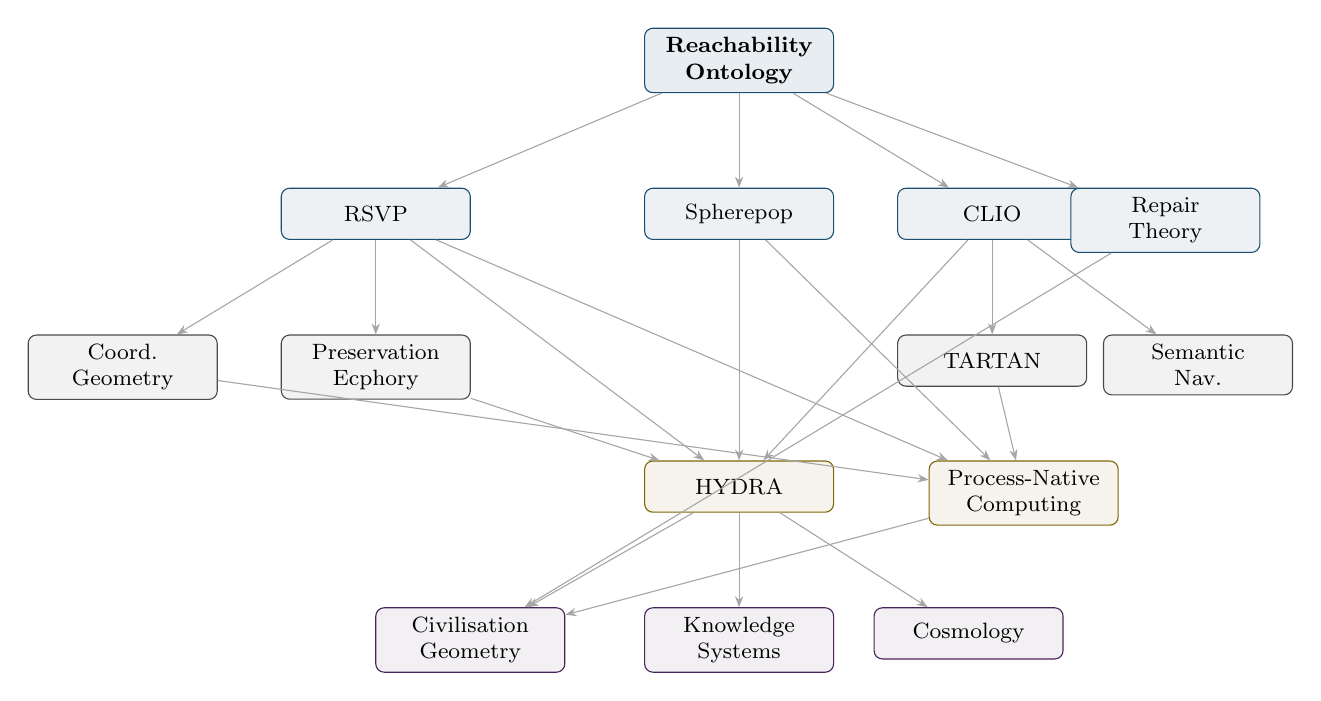
\begin{tikzpicture}[
  node distance=1.2cm and 1.4cm,
  every node/.style={font=\footnotesize, align=center},
  box/.style={draw, rounded corners=3pt, minimum width=2.4cm,
              minimum height=0.65cm, fill=lightbg},
  foundation/.style={box, draw=rsvpblue, fill=rsvpblue!10, font=\footnotesize\bfseries},
  primary/.style={box, draw=rsvpblue, fill=rsvpblue!8},
  secondary/.style={box, draw=formalismgray, fill=formalismgray!7},
  integrative/.style={box, draw=integgold, fill=integgold!8},
  applied/.style={box, draw=applviolet, fill=applviolet!7},
  arr/.style={-{Stealth[length=4pt]}, gray!70}
]

% Layer 0 — Foundation
\node[foundation] (RO) {Reachability\\Ontology};

% Layer 1 — Primary theories
\node[primary, below left=1.2cm and 2.2cm of RO] (RSVP) {RSVP};
\node[primary, below=1.2cm of RO] (Sph) {Spherepop};
\node[primary, below right=1.2cm and 0.8cm of RO] (CLIO) {CLIO};
\node[primary, below right=1.2cm and 3.0cm of RO] (RT) {Repair\\Theory};

% Layer 2 — Secondary formalisms
\node[secondary, below left=1.2cm and 0.8cm of RSVP] (CG) {Coord.\\Geometry};
\node[secondary, below=1.2cm of RSVP] (PE) {Preservation\\Ecphory};
\node[secondary, below=1.2cm of CLIO] (TAR) {TARTAN};
\node[secondary, below right=1.2cm and 0.2cm of CLIO] (SN) {Semantic\\Nav.};

% Layer 3 — Integrative
\node[integrative, below=2.8cm of Sph] (HYDRA) {HYDRA};
\node[integrative, below right=2.8cm and 1.2cm of Sph] (PNC) {Process-Native\\Computing};

% Layer 4 — Applied
\node[applied, below left=1.2cm and 1.0cm of HYDRA] (CivG) {Civilisation\\Geometry};
\node[applied, below=1.2cm of HYDRA] (Know) {Knowledge\\Systems};
\node[applied, below right=1.2cm and 0.5cm of HYDRA] (Cosm) {Cosmology};

% Edges: Foundation → Primary
\draw[arr] (RO) -- (RSVP);
\draw[arr] (RO) -- (Sph);
\draw[arr] (RO) -- (CLIO);
\draw[arr] (RO) -- (RT);

% Edges: Primary → Secondary
\draw[arr] (RSVP) -- (CG);
\draw[arr] (RSVP) -- (PE);
\draw[arr] (CLIO) -- (TAR);
\draw[arr] (CLIO) -- (SN);

% Edges: multiple parents → Integrative
\draw[arr] (RSVP)  -- (HYDRA);
\draw[arr] (Sph)   -- (HYDRA);
\draw[arr] (CLIO)  -- (HYDRA);
\draw[arr] (PE)    -- (HYDRA);
\draw[arr] (RSVP)  -- (PNC);
\draw[arr] (Sph)   -- (PNC);
\draw[arr] (TAR)   -- (PNC);
\draw[arr] (CG)    -- (PNC);

% Edges: Integrative → Applied
\draw[arr] (HYDRA) -- (CivG);
\draw[arr] (HYDRA) -- (Know);
\draw[arr] (HYDRA) -- (Cosm);
\draw[arr] (PNC)   -- (CivG);
\draw[arr] (RT)    -- (CivG);

\end{tikzpicture}
\end{center}

\bigskip

The following sections describe each layer in turn. A full framework-by-framework reference following a standard template is provided in the Appendix.

\section{Layer One: Foundational Ontology}

\subsection{Reachability Ontology}

Reachability Ontology is the philosophical foundation of the entire program.
It does not make formal mathematical claims; instead it articulates the
ontological commitments on which all the formal frameworks depend.

The central claim is that reality is not composed of objects. It is composed
of admissible transformations, of reachable trajectories, of accessible
futures. Objects, entities, and stable structures are understood as frozen
processes: trajectories that have become locally stationary, or accessibility
regions that have persisted long enough to acquire the appearance of
substance.

This inversion has consequences at every level of the program. It means that
the primary question in any domain is not \emph{what exists here?} but
\emph{what can be reached from here?} Spatial proximity is replaced by
reachability distance. Identity is replaced by trajectory continuity.
Persistence is replaced by maintained accessibility. Construction is replaced
by repair.

Reachability Ontology did not emerge as a single paper but as a convergence
of positions expressed across many works. The essays \emph{Frozen Processes},
\emph{From Preservation to Reachability}, \emph{The Geometry of Reachable
Futures}, \emph{The Secret Life of Nouns}, and \emph{Verbs Masquerading as
Nouns} collectively articulate its core commitments.

\section{Layer Two: Primary Theories}

The four primary theories each develop a major aspect of Reachability
Ontology with rigorous conceptual and, in several cases, mathematical
machinery. They are best understood as complementary rather than competing.
RSVP and CLIO answer different questions about the same underlying landscape.
Spherepop and RSVP are genuinely distinct in their fundamental objects and
operations, which is why they sit as siblings rather than in a parent-child
relationship.

One node in this layer deserves a note of caution. CLIO is classified as a
primary theory alongside RSVP, Spherepop, and Repair Theory, but it may
occupy an unusual position. Its central claim — that every description is a
projection that loses information — is not merely a claim about representation.
It is arguably an epistemological or even ontological claim of comparable
depth to Reachability Ontology's claims about trajectories and accessibility.
There is a live question about whether CLIO is a sibling of the other primary
theories or whether it should be elevated to a co-foundational role alongside
Reachability Ontology, with all observer-dependent frameworks descending from
it. The current placement reflects the working state of the architecture
rather than a settled resolution of that question.

\subsection{RSVP — Relativistic Scalar-Vector Plenum}

RSVP is the field-theoretic primary theory. It describes reality in terms of
a triple of fields: a scalar concentration field $\Phi$, a vector flow field
$\mathbf{v}$, and an entropy density field $S$. Together these define an
admissibility landscape through which processes travel, relax, and interact.

The RSVP field triple replaces the object-position ontology of classical
physics with an ontology of gradients, flows, and reachability regions.
Gravity is reinterpreted as descent through admissibility space. Cosmological
smoothing is explained through lamphrodyne relaxation rather than inflation.
Structure formation emerges from constraint erosion and differential entropy
descent.

RSVP is also the framework with the most developed associated formalization
program. Derived algebraic geometry, AKSZ and BV quantization, shifted
symplectic structures, and derived sigma model techniques have all been
invoked to give RSVP rigorous mathematical expression. These formalization
programs remain open and are detailed separately in Section~\ref{sec:formal}.

Major works include \emph{The Admissibility Field}, \emph{Axioms for a
Falling Universe}, \emph{Three Smoothing Mechanisms in Early Cosmology}, and
\emph{Constraint-Compatible Continuity Binding}.

\subsection{CLIO — Constraint-Leveraged Inference and Optimisation}

Where RSVP asks about the structure of the underlying possibility space, CLIO
asks what happens when a finite observer, agent, model, institution, or
measurement process encounters that space and projects it into a
lower-dimensional representation. The two questions are complementary and
neither subsumes the other.

A useful way to understand the epistemic situation CLIO addresses is what
might be called the Noun Fallacy: throughout history, dynamic processes are
frozen into snapshots by epistemic compression, and those snapshots are
mistaken for the actual territory. Reality is a landscape of constant
transformations; compression freezes the dynamic flow; and we then take the
label for the reality. CLIO is the theory of that compression — of what
must be discarded, what can be preserved, and what it would mean for an
observer to act ethically within those constraints.

CLIO's central claim is that abstraction is reduction: specifically, the
completion of necessary inner computation so that outer complexity can grow
without conflict. This thesis is developed formally through several
converging lines of argument. In lambda calculus, beta reduction eliminates
internal dependencies until a stable surface value emerges that can compose
without interference. Reynolds's parametricity theorem shows that polymorphic
functions cannot inspect their type arguments, forcing invariance through
reduction. In category theory, objects have no internal structure accessible
to the morphisms of the category: abstraction is the collapse of all
distinctions not preserved by composition. In Null Convention Logic, signal
stabilisation is the moment of abstraction — ongoing computation is treated
as a temporary whole until its parts collapse into determinate values. The
Curry-Howard correspondence identifies cut elimination with program execution,
making proof normalisation another instance of the same pattern.

These formally distinct processes share one invariant: inner complexity is
resolved to allow coherent outer composition. The quality of an abstraction
is therefore measured not by how much it simplifies but by which structural
invariants it preserves. CLIO distinguishes two modes. Ethical abstraction
acknowledges its own incompleteness, signals omitted complexity, preserves
admissibility, and allows the underlying reality to veto the simplification.
Extraction is the pathological form: treating the projection as the territory,
discarding admissibility-critical constraints, and confusing efficiency with
truth. This distinction connects CLIO directly to Repair Theory — extraction
is what occurs when a CLIO projection is mistaken for the territory and
admissibility is destroyed; repair is the restoration of what extraction
removed.

Major works include \emph{Hidden Manifolds}, \emph{Abstraction as Reduction},
and relevant sections of \emph{The Admissibility Field}.

\subsection{Spherepop}

Spherepop is the event-theoretic primary theory. It describes the formation,
collapse, refusal, binding, and persistence of local structures. Its
fundamental objects are not fields or gradients but events: formation events,
collapse events, binding events, refusal events, and the residues those events
leave behind.

The deepest distinction between Spherepop and RSVP is ontological. RSVP is
field-theoretic and describes reality through continuous variation across
extended regions. Spherepop is event-theoretic and describes reality through
discrete transitions that alter the set of accessible futures. The two
frameworks communicate: RSVP fields provide the landscape within which
Spherepop events occur, and Spherepop events may be interpretable as
singularities or phase transitions in RSVP fields. But the relationship
between them is one of the most important open problems in the program, and
neither framework straightforwardly reduces to the other.

A person who encountered Spherepop first could reconstruct many of its core
claims without ever encountering RSVP. The reverse is equally true. This
independence is why they sit as siblings at the primary theory layer.

Beyond the core event primitives, Spherepop has developed several
subsidiary positions. The refusal event is not a failure mode but an
autonomous primitive with its own formal properties. Irreversibility is
structural: certain collapse events cannot be undone, and this
irreversibility is a feature of the system rather than a limitation of the
observer. Time is forkable: a system can maintain multiple diverging
execution histories simultaneously, with merge and rebase operations
governing how those histories reconcile. Identity is constituted by event
history rather than by substance or persistence of parts. Scope is
geometric: the boundary of a bubble is not a syntactic convenience but a
topological feature with consequences for what can be reached from inside
it.

What distinguishes Spherepop from the other primary theories is the degree
to which its theoretical claims have been made computationally executable
and mathematically precise. The paper \emph{Structured Irreversibility}
establishes that the Spherepop category $\mathbf{SP}$ is initial in the
category of entropy-decreasing symmetric monoidal categories
($\mathbf{EDSMC}$), and constructs a functor $F: \mathbf{SP} \to
\mathbf{RSVP}$ that maps Spherepop's discrete commitment dynamics into
RSVP's continuous field dynamics with explicit entropy-slack witnesses.
This resolves the previously open question about the RSVP-Spherepop
interface: $\mathbf{SP}$ is the source of irreversible constraint
accumulation and $\mathbf{RSVP}$ is the target of smooth coherence
redistribution, connected by a structure-preserving map respecting entropy
monotonicity.

Spherepop has also been shown to be computationally universal. The full
Spherepop Calculus (SPC) subsumes simply-typed lambda calculus, Turing
machines, boolean circuits, neural feedforward dynamics, and probabilistic
lambda calculus via compositional translations. Each classical reduction
step is interpretable as a discrete geodesic in the RSVP-Ising energy
landscape, connecting computation to physics at the level of individual
steps rather than only at the architectural level.

The \emph{Joy of Spherepop} introduced the meld operator: a constrained
quotient over parallel histories that resolves distinctions incompatible
across them without reducing optionality in the same way as pop. Meld is
governed by explicit semantic merge policies separating what is synthesised
from how synthesis proceeds. This adds a sixth primitive to the canonical
set alongside pop, refuse, bind, and collapse.

The \emph{Autonomy of Refusal} develops the thesis that refusal is not a
failure mode but an autonomous primitive with formal properties
distinguishing it from preference change, negation, or
multi-objective optimisation. A non-representability theorem proves that
refusal cannot be represented as utility maximisation over a fixed
state-action-utility triple without encoding event-history as a primitive
state variable. Governance of scalable systems is reconceived as
exogenous refusal: the reintroduction of suspension capacity from outside
the system.

\emph{Active Geodesic Inference} establishes Spherepop as the natural
execution substrate for intelligence understood as maintenance of low-action
admissible histories, connecting it formally to HYDRA and to RSVP through
the Gibbs bond selection and synchronisation axioms.

The repository includes a full compiler in C with lexer, parser, runtime,
bytecode virtual machine, geometry subsystem, and a sheaf semantics layer;
multi-language prototypes in Python, Haskell, Racket, and Forth; a
shell-based event log system with overlay, fork, merge, rebase, and replay
operations; and a visualizer. Example programs in the compiler repository
execute claims from CLIO, Preservation/Ecphory, and Semantic Navigation
directly in Spherepop syntax, establishing it as a working executable
language for expressing and testing claims from the broader program. The
Spherepop OS document sketches how an operating system organised entirely
around Spherepop event primitives would behave, anticipating the AyeOS
project in the adjacent ecosystem.

The major theoretical works include \emph{Spherepop: Geometry, Cognition,
and the Transparency of Computation} alongside a substantial essay corpus
detailed in the Research Corpus section.

\subsection{Repair Theory}

Repair Theory begins with an inversion: rather than explaining persistence as
a consequence of initial construction, it treats repair as the more
fundamental category. Persistence is explained by active maintenance of
admissible states. Construction, on this view, is explained by repair
relations rather than the reverse.

The framework defines a repair relation, specifies conditions for restoration
geometry and repair latitude, and connects these to civilisational,
biological, linguistic, and computational examples. Its central claim is that
many apparently disparate domains — organism maintenance, institutional
resilience, document survival, knowledge accessibility — share a common
structure that is invisible when persistence is taken for granted and becomes
visible only when failure and repair are placed at the center.

Repair Theory began as an application of RSVP and Reachability Ontology but
has increasingly developed independent claims. The moment a repair relation is
defined as a primitive rather than derived concept, the theory acquires a
status comparable to the other primary frameworks.

The major work is \emph{Repair as a Fundamental Category}.

\section{Layer Three: Secondary Formalisms}

The secondary formalisms are mathematical and operational frameworks that
extend, connect, or operationalise the primary theories. They make stronger
formal claims than the primary theories in specific domains, but their
foundational commitments are inherited rather than independent.

\subsection{TARTAN}

TARTAN addresses the problem of constraint preservation under recursive
decomposition. When a complex system is analysed by breaking it into
components, the constraints that make the original system coherent are at risk
of being lost or violated at the level of the components. TARTAN provides a
tiling framework that ensures structural continuity across scales.

It connects most directly to CLIO on the question of how projected
representations can preserve the constraints of the systems they project, and
to RSVP on the question of how admissibility regions behave under
decomposition. It frequently appears as infrastructure in contexts where
multi-scale reasoning is required.

\subsection{Coordination Geometry}

Coordination Geometry began as an application but has grown into a hybrid
theory occupying the boundary between formal mathematics and empirical
science. It generalises synchronisation phenomena across neural systems,
distributed computation, antenna arrays, ecological networks, and collective
cognition.

Its connection to Kuramoto synchronisation, neuromorphic hardware, and
empirical biology gives it an empirical grounding the other frameworks
largely lack. At the same time, its claim that coupled systems discover and
maintain admissible coordination regions is a formal contribution that
extends RSVP dynamics into the domain of collective behaviour.

The major work is \emph{Coordination Geometry as a General Principle of
Adaptive Computation}.

\subsection{Active Geodesic Inference}

Active Geodesic Inference (AGI) is classified here as a fifth primary theory,
elevated from secondary formalism status. The basis for this elevation is that
it makes its own ontological claims — about the nature of intelligence, the
structure of semantic dynamics, and the relationship between action minimisation
and admissibility — that are independently statable, formally precise, and not
derivable from any single upstream framework. It recovers the RSVP Hamiltonian
from semantic axioms rather than importing it, and it introduces objects
(semantic isomers, geodesic width, action stability) that do not appear in any
other framework.

AGI defines intelligence formally as the capacity of a system to remain within
a family of dynamically admissible, low-action histories by actively reshaping
its configuration space's geometry. This definition is domain-invariant: it
applies equally to reasoning within an episode, learning within a lifetime, and
evolution across generations.

The framework rests on six axioms. Stationarity asserts that semantic dynamics are governed by an extremal principle selecting paths geodesically in a metric induced by a Lagrangian density. Entropy monotonicity asserts a thermodynamic arrow in semantics, encoding irreversibility at the operational level. Gibbs bond selection governs admissible interactions between semantic loci through an energy-based distribution, formalising attention as energetic bond selection. Multi-component synchronisation asserts that coherent reasoning is a synchronisation phenomenon rather than scalar optimisation. Isomeric multiplicity asserts that the variational problem admits multiple distinct stationary histories with equivalent external observables --- semantic isomers --- explaining why averaging over internally distinct reasoning trajectories degrades performance. The sixth axiom ties these together as a history-indexed, variationally governed, thermodynamically oriented, Gibbs-bonded, synchronisation-coupled dynamics.

The framework recovers the RSVP Hamiltonian as a concrete realization of the second axiom. Spherepop provides the execution calculus: its irreversible, scope-based semantics enforce history sensitivity and prevent incoherent superposition by construction, making it a natural substrate for active geodesic inference. HYDRA's cognitive architecture is the integrative realisation.

Active Geodesic Inference generates empirically testable predictions including: geodesic width predicts robust generalisation; reasoning failures manifest as phase transitions rather than smooth degradation; non-distillability of reasoning models correlates with internal isomeric multiplicity; and learning improves curvature before accuracy.



This framework addresses the long-term accessibility of information and the
conditions under which retrieval remains possible. It distinguishes between
persistence (the physical survival of a structure) and reachability (the
capacity to activate or retrieve it). Ecphoric activation describes the
threshold phenomena by which stored patterns are brought back into active
use.

The framework connects to RSVP through admissibility landscapes interpreted
as retrieval landscapes, to CLIO through the conditions on semantic
sufficiency that allow compressed representations to support later
reactivation, and to Spherepop through the residues left by collapse events,
which function as the raw material of memory.

\subsection{Semantic Navigation and Preference Fields}

This framework reconceives search and information retrieval as navigation
through a geometric possibility space. Preference fields define attractors
and repellers in semantic manifolds; admissibility filtering constrains which
trajectories are accessible; retrieval becomes trajectory selection rather
than lookup.

The framework draws directly on CLIO for its treatment of semantic manifolds
and on RSVP for its treatment of admissibility. It has produced practical
tools including EmbedFilter and related semantic manifold implementations.

\section{Layer Four: Integrative and Applied Frameworks}
\label{sec:integrative}

\subsection{HYDRA}

HYDRA is the most fully developed integrative framework and the first
large-scale attempt to operationalize multiple primary theories
simultaneously. This distinguishes it sharply from frameworks that merely
extend a single parent theory. It requires inputs
from at least RSVP, CLIO, Spherepop, and Preservation/Ecphory simultaneously.
Its purpose is to explain intelligence as the interaction of multiple
constraint-processing systems operating on admissibility landscapes.

HYDRA is not an application of any single primary theory. It is a synthesis:
a cognitive architecture that becomes possible only after several lower-level
theories have been developed sufficiently to provide its components. The
migration of RSVP Consciousness Dynamics into HYDRA, along with contributions
from Spherepop's event calculus, CLIO's projection operators, and
Preservation/Ecphory's retrieval framework, illustrates how integrative
frameworks absorb and consolidate earlier programs.

\subsection{Process-Native Computing}

Process-Native Computing applies the philosophical commitments of
Reachability Ontology to software architecture and operating system design.
It draws on Spherepop for its event-theoretic computational primitives, on
TARTAN for constraint-preserving decomposition, and on Coordination Geometry
for synchronisation mechanisms. The influence of Karl Fant, Null Convention
Logic, and Unix pipeline philosophy provides external intellectual anchors.

Its central claim is that computers should be organised around propagating
processes rather than applications and files. State, persistence, and identity
are reconceived in terms compatible with the broader ontological commitments
of the program.

\subsection{Civilisation and Institutional Geometry}

This domain application uses Repair Theory, RSVP, and elements of
Coordination Geometry to analyse social, economic, and institutional systems.
Markov boundaries define the scope of institutional action. Coordination
costs are interpreted as admissibility constraints. Fiscal reachability
extends the reachability framework to public finance. Undo stacks and
institutional repair are central organisational concepts.

Major works include \emph{Civilisation's Undo Stack}, \emph{Fiscal
Reachability and the Geometry of Public Finance}, \emph{Proxy Permanence
Failure}, and \emph{Broken Tools for a Breaking World}.

\section{The RSVP Formalization Programs}
\label{sec:formal}

The formalization programs associated with RSVP deserve separate treatment
because they are neither complete nor abandoned. They represent an ongoing
effort to give the primary theories rigorous mathematical expression using
modern tools from algebraic geometry and quantum field theory.

Active formalization programs include the derived algebraic geometry
framework, which uses derived stacks, cotangent complexes, and deformation
theory to model RSVP field configurations; the AKSZ/BV quantization program,
which constructs a sigma-model formulation of RSVP and develops a quantized
version of the entropy and flow fields; and the derived sigma model work,
which treats baryon flows and entropy fields as maps into derived moduli
spaces.

\emph{Holonomic Space: Admissibility and Reconstruction} occupies a
distinctive position within the formalization layer. Unlike the derived
geometry and quantization programs, which approach RSVP from the direction
of modern mathematical physics, Holonomic Space approaches it from the
direction of variational dynamics, sheaf theory, and observational programs
for modelling cosmology and measurement through local recursive persistence.
Its emphasis on reconstruction — on how a system's admissible states can be
recovered from local observations — connects it directly to both CLIO and
Preservation/Ecphory, giving it a broader theoretical footprint than the
other formalization programs. It is best classified as an independent
formalization strand rather than a subprogram of derived geometry.

The RSVP Field Simulator and the Admissibility Log constitute the
computational infrastructure of the formalization layer. The simulator
implements the $(\Phi, \mathbf{v}, S)$ field dynamics in a testable
environment; the log provides event-sourced record-keeping for admissibility
computations and their revision history.

These programs are classified as RSVP infrastructure rather than independent
frameworks. Their purpose is to sharpen the primary theories rather than
generate new ontological claims.

\section{Domain Applications and Peripheral Investigations}

\subsection{Ecological Network Dynamics}

\emph{The Geometry of Rewiring} applies admissibility thinking to ecological
resilience, reinterpreting it as the conservation of transformability: the
preservation of navigable future paths within an ecological network rather
than the maintenance of any particular state. This was one of the earliest
demonstrations that the admissibility framework could transfer across domains
outside cosmology and cognition, and it anticipates many of the structural
features of Civilisation and Institutional Geometry.

\subsection{Pedagogy}

\emph{Calculus as the Geometry of Relationship and Controlled Change} belongs
to the pedagogical layer. Its central move — reframing calculus as a language
for transformation rather than a collection of computational techniques —
expresses the same commitment to process and trajectory that runs through the
theoretical frameworks. It may serve as the most accessible entry point into
the broader program for readers without prior exposure to the theoretical
vocabulary.

\subsection{Peripheral Investigations}

\emph{The Stone Piano Hypothesis}, which investigates whether the
176,500-year-old Neanderthal ring structures in Bruniquel Cave functioned as
intentional lithophones exploiting the acoustic properties of speleothems,
does not derive from the Admissibility Program and does not feed back into
it in any direct theoretical way. It is classified here as a domain
investigation in archaeological acoustics — a research interest maintained
in parallel with the theoretical program rather than integrated into it.

\section{The Adjacent Ecosystem: 8b.IS and its Stack}

The 8b.IS project is an independent research and engineering effort whose
relationship to the Flyxion program is one of deep intellectual
cross-pollination rather than derivation. 8b.IS has developed its own stack
of four interconnected projects — MEM|8, AyeOS, Phoenix Protocol, and Marine
— each of which draws heavily on Flyxion theoretical vocabulary while
developing it in engineering directions that the core program does not itself
pursue.

The boundary between the two programs is real but porous. The Flyxion program
generates theoretical frameworks; 8b.IS realises those frameworks as
operating system architecture, memory physics, stability protocols, and
admissibility filters. The influence runs primarily from Flyxion outward, but
the engineering work of 8b.IS has in several cases sharpened and extended the
theoretical claims, particularly around MEM|8's wave-mechanical memory model
and Marine's tangent constraint formalism.

\subsection*{8b.IS}

8b.IS focuses on data structures and systems that resist compression, preserve
information under adversarial encoding pressure, and maintain structural
constraints across transmission and storage. Its vocabulary overlaps
substantially with RSVP and CLIO but follows its own research trajectory.

\subsection*{MEM|8}

MEM|8 is a wave-mechanical memory architecture in which memory is not stored
as static data but as active, interfering wave packets propagating through an
RSVP field residue substrate. Each memory cell is characterised by five
parameters: amplitude $A = \Phi_m$ (scalar accessibility, determining
salience), frequency $\omega$ (carrying inherent semantic content), phase
$\phi = v_m$ (associative flow, determining where the memory leads), decay
$D \propto 1/S_m$ (high-entropy memories dissolve rapidly into the
background), and interference $I$ (constructive interaction with adjacent
memory cells, governing recall). The governing equation involves the gradient
of the wave entropy field: $\nabla = \frac{\partial w_{se}}{\partial t}((x)
= v^2 v_{st} x(a,y))$.

This is substantially more developed than a simple application of Spherepop
residue concepts. MEM|8 constitutes a full wave-mechanical memory physics
grounded in RSVP field dynamics, with the $(\Phi, v, S)$ triple mapping
directly onto the amplitude, phase, and decay parameters of each wave packet.
The connections to Preservation/Ecphory (accessibility thresholds), RSVP
(field residue substrate), and Spherepop (collapse residue as memory
substrate) are all active.

\subsection*{Phoenix Protocol}

Phoenix Protocol is an entropy-resistant reconstruction system that
maintains memory field coherence against dissolution. It uses Lyapunov
stability analysis — specifically the equation $\frac{\partial}{\partial t}
|x_b| = |\leq| - \alpha \|x_m\|$ — to test whether memory configurations
remain within stable attractors. A 0.73~Hz heartbeat rhythm provides
periodic coherence testing, checking the memory field against dissolution
thresholds. The protocol represents a formal treatment of what Repair Theory
calls maintaining admissibility: it is the mechanism by which the MEM|8
system detects and corrects inadmissible memory states before they propagate.

\subsection*{Marine}

Marine is the Admissibility Gate of the 8b.IS stack: an intake filter that
blocks structurally incoherent signals from entering the semantic fluid before
they reach the MEM|8 layer. It operates via tangent constraints of the form
$\angle \simeq \frac{\|}{} + \partial_b$, testing incoming signals for
geometric admissibility before they are permitted to interact with the memory
wave field. Marine is the most direct engineering realisation of the
admissibility concept in the entire ecosystem: where the Flyxion program
defines admissibility theoretically, Marine implements it as a filter.

\subsection*{AyeOS}

AyeOS is the orchestration layer of the stack. It uses sheaf-theoretic routing
governed by a functor $\mathcal{F} \equiv \bigl\{\frac{G}{1}\ X\bigr\}$, with
the operating system scheduler directing data along paths that preserve
semantic coherence across the full stack. AyeOS is best understood as an
engineering realisation of Process-Native Computing and Spherepop's event
primitives, instantiating sheaf-theoretic ideas from TARTAN and Holonomic
Space at the operating system level.

The four projects form a coherent vertical stack: Marine filters for
admissibility at intake, MEM|8 stores and retrieves via wave-mechanical
dynamics, Phoenix Protocol maintains field coherence against entropy, and
AyeOS orchestrates the whole via semantics-preserving sheaf routing.

% ============================================================
\part*{Part III\quad Open Problems}
\addcontentsline{toc}{part}{Part III: Open Problems}

\section{Major Unresolved Questions}

\subsection{The Continuous-Discrete Interface: RSVP and Spherepop}

This was the most important unresolved question in the program. \emph{Structured Irreversibility} has now provided a significant partial answer.

The paper proves that the Spherepop category $\mathbf{SP}$ --- the free symmetric monoidal entropy-decreasing rewriting category generated by the event primitives Pop, Refuse, Bind, and Collapse --- is initial in the category $\mathbf{EDSMC}$ of entropy-decreasing symmetric monoidal categories. It then constructs a symmetric monoidal functor $F: \mathbf{SP} \to \mathbf{RSVP}$ into a smooth realization category whose objects are manifolds equipped with coherence potential $\Phi$, velocity field $v$, and entropy density $S$, and whose morphisms carry explicit entropy-slack witnesses.

This functor resolves the interface question in a specific direction: Spherepop's discrete combinatorial constraint accumulation maps into RSVP's continuous coherence redistribution. The two frameworks are not dual descriptions of the same structure, nor is one a coarse-graining of the other. Instead, $\mathbf{SP}$ is the source category of irreversible commitments and $\mathbf{RSVP}$ is the target category of smooth field dynamics, connected by a structure-preserving map that respects entropy monotonicity.

What remains open is whether $F$ is faithful (whether distinct Spherepop histories always produce distinct RSVP realizations), whether the category admits a compact-closed extension supporting a duality between commitment and co-commitment, and whether the functor lifts to a quantum or unistochastic extension connecting to the probabilistic Spherepop calculus.

\subsection{Projection and Intrinsic Structure: The CLIO Problem}

CLIO raises a question it cannot answer within its own framework: how much of
the structure we observe in a domain is intrinsic to that domain, and how
much is introduced by the act of projection? If every observer constructs a
compressed representation of reality, there is a risk that the structures
reported by observers are partly artefacts of their projection operators
rather than features of the underlying admissibility landscape.

Resolving this requires either a theory of projection-invariant structure
within CLIO, or an account of how RSVP fields can be accessed without the
mediating distortion of CLIO projection. Neither account currently exists.

\subsection{Repair and Thermodynamics}

Repair Theory claims that repair is more fundamental than construction. But
this claim sits in tension with standard thermodynamic reasoning, which
treats the maintenance of low-entropy states as a cost requiring external
energy input. The question is whether repair can be derived from admissibility
dynamics — perhaps as a directed trajectory in RSVP field space toward
restored admissibility — or whether it must be taken as a genuinely primitive
category irreducible to field dynamics.

If repair is derivable, Repair Theory becomes a special case of RSVP applied
to persistence. If it is primitive, Repair Theory retains its status as an
independent primary framework with consequences for thermodynamics rather than
consequences derived from it.

\subsection{Coordination and Meaning}

Coordination Geometry raises the question of whether semantic structure can
emerge purely from coordination dynamics. If sufficiently complex patterns of
synchronisation and desynchronisation among coupled systems can generate
stable categories, reference, and inference, then meaning may be a
coordination phenomenon rather than a representational one. This would
connect Coordination Geometry directly to CLIO and might allow the two
frameworks to be unified under a common account of how structured information
emerges from dynamic processes.

\subsection{Preservation and Reachability}

The mathematical relationship between persistence, accessibility, and
retrieval remains incompletely characterised. Preservation/Ecphory
distinguishes between physical survival and reachability, but a precise
formal account of what determines whether a stored pattern crosses the
ecphoric activation threshold is not yet available. This question connects to
RSVP through admissibility landscape topology, to CLIO through semantic
sufficiency conditions, and to Spherepop through the structure of collapse
residues.

\subsection{The Umbrella Question}

The program as a whole circles around a question that may constitute its
ultimate research target:

\begin{quote}
\itshape
How do stable structures emerge, persist, transform, and remain reachable
within a universe fundamentally composed of processes rather than things?
\end{quote}

Nearly every major framework can be understood as an attack on this question
from a different direction. The open problem at the highest level is whether
the individual answers can be assembled into a unified theoretical statement
that is not merely a summary of its components but a genuinely novel claim
about the nature of admissible reality.

\section{The Central Conjecture of the Admissibility Program}

The preceding sections have traced the historical origins of the program,
mapped its dependency architecture, and catalogued its open problems. It
remains to state, as explicitly as the current state of the work permits, the
single overarching thesis that the entire program is attempting to establish.

The conjecture is this.

\begin{quote}
\itshape
Across physics, cognition, memory, computation, ecology, and civilisation,
the primary explanatory object is neither substance nor information but the
structure of admissible transformations. Stable entities emerge as
maintained regions of admissibility. Persistence is the preservation of
admissible trajectories. Repair is the restoration of lost admissibility.
Cognition is navigation through admissibility landscapes. Meaning is the
result of coordination within admissible synchronisation regions. Institutions
are mechanisms for maintaining collective admissibility across time.
\end{quote}

This conjecture has a number of important features.

It is domain-invariant. The same structural claim applies to cosmological
field dynamics, to neural memory retrieval, to ecological resilience, to
software architecture, to institutional governance, and to the long-term
survival of knowledge. The domains differ; the explanatory structure is
shared.

It is process-first. The objects that populate ordinary scientific and
philosophical descriptions — particles, mental states, organisms, institutions,
documents — appear here not as primitives but as derived categories:
stabilised processes, maintained accessibility regions, frozen trajectories.
The primary vocabulary is transformation, admissibility, and reachability
rather than object, property, and relation.

It is repair-centred. The standard picture of reality privileges construction:
things come into existence through assembly, combination, or generation. The
Admissibility Program inverts this. Things persist through repair. The
explanatorily prior category is not how something was built but how its
admissibility is maintained against the constant pressure of degradation,
constraint erosion, and trajectory loss.

It makes contact with experience. The conjecture did not arise from pure
speculation. It was generated by sustained engagement with physical systems
— construction, electrical work, plumbing, property rehabilitation — in which
the practical question is never the ideal design but always the available
transformation: what can be done from here, within these constraints, without
destroying the continuity that makes the system repairable at all. The
conjecture is in that sense empirically grounded in a practice, even before
it is tested against formal theory.

The conjecture is not yet proven. Several of its components — the
relationship between RSVP and Spherepop, the status of CLIO as primary theory
or co-foundation, the derivability of repair from admissibility dynamics —
remain genuinely open. The document has been honest about these tensions
rather than resolving them prematurely. What can be said is that the
conjecture has survived contact with a large number of domains, has generated
productive research programs in each of them, and has not yet been
contradicted by any of them.

That is enough to warrant calling it a research program.

% ============================================================
\section{The Architecture in Retrospect}

The following table summarises the current status of each framework in the
program. Status reflects the degree to which a framework has produced stable
formal claims, worked examples, and cross-framework integration, rather than
merely a count of associated papers.

\bigskip

\begin{center}
\small
\begin{tabular}{llll}
\toprule
\textbf{Layer} & \textbf{Framework} & \textbf{Status} & \textbf{Primary Integration Points} \\
\midrule
Ontology & Reachability Ontology & Mature & All primary theories \\
Primary Theory & RSVP & Mature & CLIO, Spherepop, Coord.\ Geometry \\
Primary Theory & Spherepop & Mature & RSVP ($F$: SP$\to$RSVP), HYDRA, PNC \\
Primary Theory & CLIO & Mature & TARTAN, Semantic Navigation, HYDRA \\
Primary Theory & Repair Theory & Developing & Civilisation Geometry, RSVP \\
Primary Theory & Active Geodesic Inference & Developing & RSVP, Spherepop, CLIO, HYDRA \\
Secondary & TARTAN & Developing & CLIO, RSVP, Process-Native Computing \\
Secondary & Coordination Geometry & Developing & RSVP, HYDRA, PNC \\
Secondary & Preservation/Ecphory & Developing & RSVP, CLIO, Spherepop, HYDRA \\
Secondary & Semantic Navigation & Developing & CLIO, RSVP \\
Formalization & Holonomic Space & Active & RSVP, CLIO, Preservation/Ecphory \\
Formalization & Derived Geometry / AKSZ & Active & RSVP \\
Integrative & HYDRA & Emerging & RSVP, CLIO, Spherepop, Preservation, AGI \\
Integrative & Process-Native Computing & Emerging & Spherepop, TARTAN, Coord.\ Geometry \\
Applied & Civilisation Geometry & Emerging & Repair Theory, RSVP, Coord.\ Geometry \\
\bottomrule
\end{tabular}
\end{center}

\bigskip

The four primary theories can also be compared directly across three dimensions —
their core domain, fundamental primitive, and relationship to entropy — in a
way that makes their complementarity visible at a glance.

\bigskip
\begin{center}
\small
\begin{tabular}{p{2.8cm}p{2.8cm}p{2.8cm}p{4.5cm}}
\toprule
\textbf{Theory} & \textbf{Core Domain} & \textbf{Fundamental Primitive} & \textbf{Relationship to Entropy} \\
\midrule
RSVP & Cosmology / Physics & Continuous fields $(\Phi, v, S)$ & Gravity is entropy descent; structure formation via constraint erosion \\
\addlinespace
Spherepop & Computation & Discrete events (Pop, Refuse, Bind, Collapse) & Initial in entropy-decreasing monoidal categories; $F: \mathbf{SP}\to\mathbf{RSVP}$ \\
\addlinespace
CLIO & Epistemology / Observation & Projection operators & Pathological extraction destroys system admissibility constraints \\
\addlinespace
Repair Theory & Persistence & The repair relation & Fighting thermodynamic degradation to maintain repair latitude \\
\addlinespace
Active Geodesic Inference & Intelligence & Semantic isomers & Intelligence is maintenance of low-action admissible histories \\
\bottomrule
\end{tabular}
\end{center}
\bigskip

Beyond the dependency graph, the architecture can be read along three distinct
thematic axes that cut across the layer model. These axes are not alternatives
to the dependency structure but complementary perspectives on it.

\begin{center}
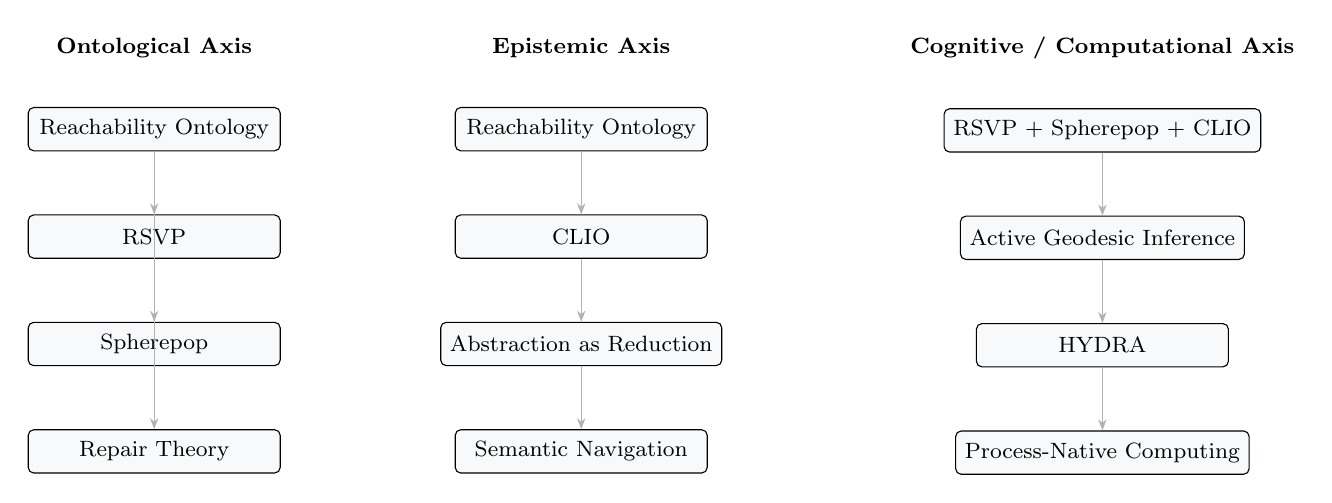
\begin{tikzpicture}[
  node distance=0.8cm and 2.8cm,
  every node/.style={font=\footnotesize, align=center},
  axbox/.style={draw, rounded corners=2pt, fill=lightbg, minimum width=3.2cm, minimum height=0.55cm},
  axlabel/.style={font=\footnotesize\bfseries},
  arr/.style={-{Stealth[length=4pt]}, gray!60}
]

% Axis 1: Ontological
\node[axlabel] (A1) {Ontological Axis};
\node[axbox, below=0.5cm of A1] (a1n1) {Reachability Ontology};
\node[axbox, below=of a1n1] (a1n2) {RSVP};
\node[axbox, below=of a1n2] (a1n3) {Spherepop};
\node[axbox, below=of a1n3] (a1n4) {Repair Theory};
\draw[arr] (a1n1) -- (a1n2);
\draw[arr] (a1n1) -- (a1n3);
\draw[arr] (a1n1) -- (a1n4);

% Axis 2: Epistemic
\node[axlabel, right=of A1] (A2) {Epistemic Axis};
\node[axbox, below=0.5cm of A2] (a2n1) {Reachability Ontology};
\node[axbox, below=of a2n1] (a2n2) {CLIO};
\node[axbox, below=of a2n2] (a2n3) {Abstraction as Reduction};
\node[axbox, below=of a2n3] (a2n4) {Semantic Navigation};
\draw[arr] (a2n1) -- (a2n2);
\draw[arr] (a2n2) -- (a2n3);
\draw[arr] (a2n3) -- (a2n4);

% Axis 3: Cognitive/Computational
\node[axlabel, right=of A2] (A3) {Cognitive / Computational Axis};
\node[axbox, below=0.5cm of A3] (a3n1) {RSVP + Spherepop + CLIO};
\node[axbox, below=of a3n1] (a3n2) {Active Geodesic Inference};
\node[axbox, below=of a3n2] (a3n3) {HYDRA};
\node[axbox, below=of a3n3] (a3n4) {Process-Native Computing};
\draw[arr] (a3n1) -- (a3n2);
\draw[arr] (a3n2) -- (a3n3);
\draw[arr] (a3n3) -- (a3n4);

\end{tikzpicture}
\end{center}

\bigskip

Several observations follow from this map.

\textit{What is primary.} The mature layer — Reachability Ontology, RSVP,
Spherepop, CLIO — is where the program's most stable and independently
defensible claims live. Active Geodesic Inference is now listed as a fifth
primary theory at developing status. Its six axioms, its independent notion
of intelligence, its reconstruction of the RSVP Hamiltonian, and its
empirically testable predictions distinguish it from a secondary formalism.
The boundary it has crossed is the one separating frameworks that apply or
extend existing concepts from frameworks that make their own ontological
claims.

\textit{What is derivative.} The secondary and integrative frameworks are
not independent. TARTAN requires CLIO. Coordination Geometry requires RSVP.
HYDRA requires all primary theories simultaneously. None of these can
survive if their upstream dependencies are abandoned.

\textit{What is mature.} A framework is mature in this program when three
conditions hold: its central claim is independently statable, its formal
objects are defined precisely enough to support proofs, and it has been
tested against at least two independent domains. By that criterion, the four
classical primary theories and Reachability Ontology are mature. The functor
$F: \mathbf{SP} \to \mathbf{RSVP}$ proved in \emph{Structured Irreversibility}
represents a step-change in maturity for both Spherepop and their
relationship.

\textit{What is speculative.} The most speculative elements are the
consciousness and cognition claims in HYDRA and Active Geodesic Inference,
the governance architecture in \emph{The Forkability of Time}, and the
amplitwistor extension of Spherepop in \emph{Spherepop Foundations}. These
are productive speculations — they generate testable predictions and formal
obligations — but they have not yet been subjected to the cross-domain stress
testing that the mature frameworks have.

\textit{The three thematic axes.} Beyond the dependency graph, the architecture
can be read along three distinct intellectual lineages. The ontological axis
runs from Reachability Ontology through RSVP, Spherepop, and Repair Theory:
it answers the question of what exists and how it persists. The epistemic
axis runs from Reachability Ontology through CLIO, Abstraction as Reduction,
and Semantic Navigation: it answers the question of how finite observers
represent and navigate admissibility landscapes. The cognitive-computational
axis runs from the primary theories through Active Geodesic Inference into
HYDRA and Process-Native Computing: it answers the question of how
intelligence is constituted and implemented. The diagram below makes these
three trajectories visible alongside the dependency graph.

\textit{The major integration points.} The program has three critical joints.
The first is the RSVP-Spherepop functor, which connects the field-theoretic
and event-theoretic primary theories. The second is HYDRA, which requires
all primary theories as simultaneous inputs. The third is Active Geodesic
Inference, which reconstructs the RSVP Hamiltonian from semantic axioms,
suggesting that the field equations may be more fundamental than any
particular physical interpretation of them.

% ============================================================
\appendix
\part*{Appendix A\quad Framework Reference Guide}
\addcontentsline{toc}{part}{Appendix A: Framework Reference Guide}

\section{How to Use This Appendix}

Each entry follows a standard template: Purpose, Central Claim, Core
Objects, Relationships to Other Frameworks, Major Works, and Open Problems.
Entries are organised by layer. Within each layer, ordering is roughly by
degree of development, most developed first.

\section{Precursor Works}

\frameworkhead{Persistent Anomalies and the Geometry of Ontology Revision}{formalismgray}{Emerged from practical and theoretical engagement with data model failure,
prior to the explicit articulation of the Admissibility Program. One of the
earliest published works under the Flyxion name.}{None formally; this is a precursor document. Retroactively connected to
Reachability Ontology, Repair Theory, and CLIO.}{To develop a framework for distinguishing minor errors from fundamental
structural failures in data models, using the language of topological
obstruction and repair.}
\frameworkbody{Not all anomalies require local correction. Some represent topological
obstructions that require revision of the ontological framework itself.
Repair is the appropriate response to structural failure, not
reconstruction.}{Topological obstruction; ontology revision; structural failure; repair
threshold; admissibility of data models.}{This monograph now appears as one of the earliest explicit precursors to
Repair Theory, CLIO, and Reachability Ontology. Its obstruction vocabulary
anticipates the sheaf-theoretic strand of TARTAN. It predates the formal
articulation of the Admissibility Program but already operates within its
conceptual space.}{\emph{Persistent Anomalies and the Geometry of Ontology Revision}.}{How does the obstruction-theoretic framework developed here relate formally
to the sheaf-theoretic obstruction machinery in TARTAN? Can the ontology
revision framework be embedded within CLIO's projection-theoretic language?}

\section{Formalization Programs}

\frameworkhead{Holonomic Space}{formalismgray}{Emerged from the RSVP formalization effort as an attempt to bridge the
physical intuitions of the plenum theory with rigorous sheaf-theoretic
machinery. Developed in parallel with, rather than downstream of, the
derived algebraic geometry program.}{RSVP (primary); Reachability Ontology (philosophical); connects laterally
to CLIO and Preservation/Ecphory.}{To provide a formalization of admissibility and reconstruction using
variational dynamics, sheaf theory, and observational programs, modelling
cosmology and measurement through local recursive persistence.}
\frameworkbody{Admissible states of a system can be reconstructed from local observations
under appropriate holonomy conditions. Measurement is not passive recording
but active trajectory reconstruction within a sheaf-theoretic admissibility
structure.}{Holonomy; local recursive persistence; sheaf; variational dynamics;
observational program; admissibility reconstruction.}{Holonomic Space sits between RSVP and the derived algebraic geometry
formalization program. Its sheaf-theoretic approach connects it to TARTAN
and its reconstruction emphasis connects it to CLIO and Preservation/Ecphory.
It is best understood as an independent formalization strand with broader
theoretical footprint than the quantization programs.}{\emph{Holonomic Space: Admissibility and Reconstruction} (multi-part
monograph, in development).}{The precise relationship between holonomic reconstruction and RSVP field
recovery. Whether the observational program developed here can be used to
generate empirical predictions distinguishable from standard cosmological
models.}

\frameworkhead{Derived Algebraic Geometry Formalization}{formalismgray}{Emerged during the early RSVP-centric phase as the primary mathematical
formalization effort. Predates several of the primary theories and was
originally conceived as the route from RSVP to a rigorous quantum field
theory.}{RSVP (exclusively); AKSZ/BV Quantization (downstream).}{To express RSVP field configurations using the machinery of derived algebraic
geometry, providing a rigorous mathematical foundation for the primary
theory.}
\frameworkbody{RSVP field configurations can be modelled as points in derived moduli
spaces, with deformation theory governing the behaviour of nearby
configurations and shifted symplectic structures providing the geometric
framework for quantization.}{Derived stack; cotangent complex; shifted symplectic structure; deformation
theory; moduli space; derived moduli.}{Provides mathematical infrastructure for RSVP. Connects to the AKSZ/BV
quantization program as its immediate downstream application.}{Derived geometry and RSVP notes; \emph{Derived L-System Sigma Models}.}{Completion of the deformation-theoretic description of RSVP field space.
Relationship between derived moduli geometry and the admissibility landscape
concept.}

\frameworkhead{AKSZ/BV Quantization}{formalismgray}{Developed as a direct continuation of the derived algebraic geometry
program, once the moduli space description of RSVP fields was sufficiently
developed to support a sigma-model construction.}{Derived Algebraic Geometry Formalization (prerequisite); RSVP (target
theory).}{To construct a complete sigma-model formulation of RSVP and develop a
quantized version of the entropy and flow fields using the AKSZ formalism
and Batalin-Vilkovisky quantization.}
\frameworkbody{RSVP fields can be modelled as maps from a source manifold into a derived
target space, and the resulting sigma model can be quantized using BV methods
to yield a well-defined quantum field theory of the plenum.}{AKSZ sigma model; BV quantization; entropy field map; baryon flow; derived
target; gauge symmetry; ghost fields.}{Downstream of the derived algebraic geometry program. Connects RSVP to the
broader landscape of topological and quantum field theories.}{AKSZ/BV quantization notes; \emph{Gravity as Entropy Descent}.}{Whether the quantized RSVP theory recovers standard results in the
appropriate limits. The role of entropy field quantization in the broader
cosmological picture.}

\section{Foundational Ontology}

\frameworkhead{Reachability Ontology}{rsvpblue}{Emerged as a convergence of process-over-object intuitions accumulated
across the early RSVP work, the repair and construction practice, and
early essays on language and cognition. Was not named as a distinct
framework until several of the primary theories had already been developed.}{Practice layer (ground-floor intuitions); no formal upstream dependencies
within the theoretical graph.}{To articulate the ontological commitments on which the formal frameworks
depend, by making explicit the claim that reality consists of admissible
transformations rather than objects.}
\frameworkbody{Objects are frozen trajectories. Reality is constituted by the differential
reachability of admissible futures rather than by the intrinsic properties of
persisting substances.}{Admissible transformations; reachable futures; trajectories; accessibility
regions; frozen processes.}{All other frameworks in the program depend on this layer either directly or
transitively. RSVP provides its first field-theoretic formalisation. CLIO
provides its projection-theoretic complement. Spherepop provides its
event-theoretic complement. Repair Theory provides its persistence-theoretic
complement.}{\emph{Frozen Processes}; \emph{From Preservation to Reachability}; \emph{The
Geometry of Reachable Futures}; \emph{The Secret Life of Nouns}; \emph{Verbs
Masquerading as Nouns}.}{What is the minimal formal language capable of expressing all the
commitments of Reachability Ontology without importing the vocabulary of any
particular primary theory? Is there a unifying mathematical structure — a
category of admissible transformations, perhaps — from which RSVP, CLIO, and
Spherepop can all be derived as special cases?}

\section{Primary Theories}

\frameworkhead{RSVP}{rsvpblue}{The original and longest-running framework in the program. Began as a
cosmological field theory and expanded to encompass consciousness dynamics,
gravity, structure formation, and entropy. During the early phase of the
program it functioned as a universal attractor for nearly all other
theoretical questions.}{Reachability Ontology (philosophical foundation); practice layer
(original intuitions about constrained flow).}{To provide a field-theoretic account of admissibility dynamics in which
gravity, entropy, structure formation, and cosmological evolution are
explained through the behaviour of the $(\Phi, \mathbf{v}, S)$ field triple.}
\frameworkbody{The structure of reality at every scale can be described by the dynamics of
scalar concentration, vector flow, and entropy density fields over admissibility
landscapes. Gravity is descent through admissibility space. Cosmological
smoothing proceeds through lamphrodyne relaxation rather than inflation.}{Scalar field $\Phi$; vector flow field $\mathbf{v}$; entropy density $S$;
admissibility landscape; lamphrodyne relaxation; constraint erosion.}{RSVP is the primary field-theoretic development of Reachability Ontology.
CLIO addresses the complementary question of observer projection over RSVP
landscapes. Spherepop operates at the event-theoretic level and may describe
singularities or phase transitions within RSVP dynamics. Coordination
Geometry and Preservation/Ecphory are downstream secondary formalisms.
HYDRA, Process-Native Computing, and Civilisation Geometry are downstream
integrative or applied frameworks. The RSVP formalization programs provide
mathematical infrastructure.}{\emph{The Admissibility Field}; \emph{Axioms for a Falling Universe};
\emph{Three Smoothing Mechanisms in Early Cosmology};
\emph{Constraint-Compatible Continuity Binding}; \emph{Gravity as Entropy
Descent}.}{Resolution of the RSVP-Spherepop interface (continuous fields versus
discrete events). Completion of the AKSZ/BV quantization program. Empirical
or observational consequences distinguishing RSVP from competing cosmological
theories.}

\frameworkhead{CLIO}{cliogreen}{Emerged as the questions left unanswered by RSVP became clear: RSVP
describes the landscape, but what happens when a finite system must act on
that landscape using a compressed representation? Early abstraction essays
and the Hidden Manifolds work crystallised these concerns into a framework.
The monograph \emph{Abstraction as Reduction} developed the core thesis
through lambda calculus, Reynolds parametricity, category theory, NCL signal
stabilisation, and the Curry-Howard correspondence, establishing that
abstraction is not merely a representational tool but a structural feature
of existence.}{Reachability Ontology (philosophical); RSVP (landscape it operates over);
possibly co-foundational with Reachability Ontology — see note in
Section~\ref{sec:primary}.}{To formalise what happens when a finite observer, agent, model, or
institution projects an admissibility landscape into a lower-dimensional
representation, and to distinguish productive reduction from pathological
extraction.}
\frameworkbody{Abstraction is reduction: the completion of necessary inner computation so
that outer complexity can grow without conflict. Every description is a
projection that loses information; the quality of a description is determined
by what structural invariants it preserves. Reduction manifests differently
across domains — beta reduction in lambda calculus, cut elimination in proof
theory, signal stabilisation in NCL, morphism collapse in category theory —
but shares an invariant pattern: inner complexity is resolved to allow
coherent outer composition. Ethical abstraction acknowledges its
incompleteness, preserves admissibility, and allows the underlying reality
to veto the simplification. Extraction is the pathological form: treating
the projection as the territory, discarding crucial constraints, and
prioritising efficiency over structural fidelity.}{Projection operators; representational entropy; semantic sufficiency;
hidden manifolds; information loss; recoverability conditions; beta
reduction; parametricity; cut elimination; signal stabilisation; canonical
form; epistemic compression; ethical abstraction; extraction; constraint
set; admissible transformation; unistochastic interface matrix; geodesic
inference.}{CLIO is the projection-theoretic complement to RSVP. It inherits the
admissibility landscape from RSVP but addresses a distinct question: the
behaviour of observers rather than the behaviour of the landscape itself.
The ethical abstraction versus extraction distinction connects CLIO directly
to Repair Theory: extraction is what occurs when a CLIO projection is
mistaken for the territory and admissibility is no longer preserved; repair
is the restoration of that admissibility. TARTAN extends CLIO into recursive
decomposition. Semantic Navigation applies CLIO to information retrieval and
incorporates unistochastic interface matrices to model amplitude-level
constraints on probabilistic transitions, enabling identity-preserving
inference as geodesic evolution. HYDRA draws on CLIO's projection operators
for its cognitive architecture. CLIO's status as a primary sibling versus a
co-foundational node alongside Reachability Ontology remains an open
architectural question.}{\emph{Hidden Manifolds}; \emph{Abstraction as Reduction}; relevant sections
of \emph{The Admissibility Field}.}{The projection-invariance problem: what features of an admissibility
landscape survive arbitrary projection, and how can they be distinguished
from artefacts of the projection operator? Whether CLIO should be elevated
to a co-foundational role. The relationship between CLIO compression and
RSVP field recoverability. Whether the unistochastic constraint on interface
matrices can be derived from the admissibility conditions on RSVP fields,
which would unify the quantum-geometric and field-theoretic strands of the
program.}

\frameworkhead{Spherepop}{spherered}{Originated as a cognitive and visual language for describing nested scope
and evaluation — a way of making the geometry of computation visible through
bubble nesting rather than symbolic expression. Gradually expanded into a
general calculus for formation, collapse, residue, refusal, and
history-as-identity. Developed substantially independently of RSVP, sharing
the process-first intuition but arriving at it through a different route.
The theoretical work has been accompanied by a substantial implementation
program: a full compiler in C with its own lexer, parser, runtime, bytecode
VM, geometry subsystem, and sheaf semantics layer; prototypes in Python,
Haskell, Racket, and Forth; a shell-based event log system with overlay,
fork, merge, rebase, and replay tooling; and a visualizer. Example programs
in the compiler repository execute claims from CLIO, Preservation/Ecphory,
and Semantic Navigation directly in Spherepop syntax, establishing it as
a working executable language for the broader program.}{Reachability Ontology (philosophical foundation); no formal dependency on
RSVP — the two are siblings.}{To provide an event-theoretic account of how stable local structures form,
persist, collapse, refuse, bind, and leave residues within dynamic systems,
and to make this account computationally executable.}
\frameworkbody{Formation, collapse, binding, refusal, and residue are primitive events that
constitute the history of a system. Histories are more fundamental than
states. Identity is event history, not substance. Stable structures are
persistent accessibility regions in event history space. Refusal is an
autonomous primitive that cannot be represented as utility maximisation over
a fixed state-action-utility triple without encoding event-history as a
primitive state variable. Irreversibility is structural, not incidental.
Time is forkable. The Spherepop category $\mathbf{SP}$ is initial in the
category of entropy-decreasing symmetric monoidal categories
($\mathbf{EDSMC}$), and there exists a symmetric monoidal functor $F:
\mathbf{SP} \to \mathbf{RSVP}$ connecting discrete commitment dynamics to
continuous field dynamics. Spherepop is computationally universal,
subsuming lambda calculus, Turing machines, neural feedforward dynamics,
and probabilistic computation.}{Bubble; formation event; collapse event; refusal; binding; residue; scope;
history as primitive; collapse residue; structured irreversibility; scope
geometry; commitment calculus; temporal fork; operational mereology;
admissibility check; trajectory collapse; execution history; meld operator;
semantic merge policy; monoidal category; tensor product as parallel merge;
idempotent merge; commutative merge; morphism as geometric transformation;
coherence isomorphism; geometric region; payload; coordinate-labelled sphere;
EDSMC; entropy-slack witness; option space; commitment history; Lagrangian over
option spaces; Hamiltonian as remaining maneuverability; discrete geodesic;
semantic isomer.}{The functor $F: \mathbf{SP} \to \mathbf{RSVP}$ (\emph{Structured Irreversibility})
formally connects Spherepop and RSVP: $\mathbf{SP}$ accumulates constraints
combinatorially while $\mathbf{RSVP}$ redistributes coherence
differentially. This resolves the previously open interface question in a
specific direction without collapsing the two frameworks. The sheaf semantics
layer in the compiler connects Spherepop to TARTAN's obstruction framework.
CLIO projection and semantic navigation are already expressed as executable
Spherepop programs. Active Geodesic Inference uses Spherepop as its
execution substrate, connecting it to HYDRA and RSVP via the Gibbs bond
selection and synchronisation axioms. Process-Native Computing draws on
Spherepop event-theoretic primitives. Spherepop residues connect to
Preservation/Ecphory and, in the 8b.IS ecosystem, to MEM|8's wave-mechanical
memory. The meld operator provides a sixth primitive governing convergence of
parallel histories, relevant to Civilisation Geometry's treatment of
institutional reconciliation. The non-representability theorem for refusal
connects \emph{The Autonomy of Refusal} and \emph{Throwing the Game} to
governance theory in Civilisation Geometry.}{Monograph corpus: \emph{Spherepop: Geometry, Cognition, and the
Transparency of Computation}; \emph{Structured Irreversibility}; \emph{The
Autonomy of Refusal}; \emph{The Forkability of Time}; \emph{History as
Identity}; \emph{Scope as Geometry}; \emph{The Calculus of Commitment};
\emph{Operational Mereology}; \emph{Active Geodesic Inference}; \emph{Joy of
Spherepop}; \emph{Computation After Storage}; \emph{Computation as Semantic
Maintenance}; \emph{Event-Historical Aggregation}; \emph{Throwing the Game};
\emph{Sheaf of Flow Obstructions}; \emph{Spherepop OS}; \emph{The Geometry
of Spherepop}; \emph{The History of Spherepop}; \emph{Spherepop Trajectory
Collapse}; \emph{Spherepop Foundations}; \emph{Intelligence Explosion};
\emph{Attention as Minimal Relational Interaction}; \emph{Entropy of
Austerity}; \emph{Spherepop Calculus} (SPC with Giry monad); \emph{Spherepop
Specifications}; plus the full compiler codebase, multi-language prototype
implementations, and the Adaptive Trust Dynamics corpus.}{Whether $F: \mathbf{SP} \to \mathbf{RSVP}$ is faithful (distinct Spherepop
histories always produce distinct RSVP realizations). Whether the category
admits a compact-closed or $\ast$-autonomous extension supporting a duality
between commitment and co-commitment. Whether the functor lifts to a quantum
or unistochastic extension connecting to the probabilistic SPC. Whether the
meld operator can be derived from the existing four primitives or is
genuinely independent. Whether temporal forking in Spherepop corresponds
precisely to branching in RSVP admissibility landscapes. The relationship
between history-as-identity and Preservation/Ecphory's ecphoric activation
threshold.}

\frameworkhead{Repair Theory}{repairteal}{Has roots in the practical construction and rehabilitation work, which
repeatedly encountered systems that could not be rebuilt from scratch and
required active maintenance of continuity. First formalised as an extension
of RSVP; gradually developed independent claims. The \emph{Persistent
Anomalies} monograph is an early precursor.}{Practice layer (primary intuitive source); Reachability Ontology
(philosophical foundation); RSVP (natural formal language, though not a
strict prerequisite).}{To establish repair as a more fundamental category than construction, and to
provide a framework in which persistence across biological, social,
linguistic, and technological systems is explained by active maintenance of
admissible states.}
\frameworkbody{Persistence is not explained by construction. Construction is explained by
repair. The repair relation is a primitive that characterises how a system
returns from inadmissible states to admissible ones.}{Repair relation; restoration geometry; repair latitude; admissible state;
inadmissible state; repair infrastructure; knowledge as repair capacity.}{Repair Theory began as an extension of RSVP and Reachability Ontology but
has developed increasing independence. Its connection to thermodynamics is an
open problem that may determine whether it is a derived or primitive
framework. It contributes directly to Civilisation Geometry through the
concepts of institutional repair and civilisational undo stacks.}{\emph{Repair as a Fundamental Category}.}{Can the repair relation be derived from admissibility dynamics, or is it
irreducibly primitive? What is the relationship between repair latitude and
thermodynamic entropy production? How does repair theory apply to linguistic
and semantic structures?}

\section{Secondary Formalisms}

\frameworkhead{TARTAN}{formalismgray}{Arose from the practical problem of how multi-scale descriptions preserve
the constraints of the systems they describe. Developed in the context of
RSVP and CLIO work on admissibility under decomposition.}{CLIO (projection-theoretic parent); RSVP (admissibility landscape source);
Holonomic Space (sheaf-theoretic connection).}{To provide a framework for constraint preservation under recursive
decomposition, ensuring that structural continuity is maintained when complex
systems are analysed at multiple scales.}
\frameworkbody{Recursive decomposition need not destroy the constraints of the original
system if the decomposition respects admissibility-preserving tiling
conditions.}{Recursive tiling; constraint-preserving decomposition; structural
continuity; multi-scale reasoning; admissibility inheritance.}{TARTAN connects most directly to CLIO on the question of
projection-preserving decomposition and to RSVP on admissibility region
behaviour under subdivision. It provides infrastructure for Process-Native
Computing wherever multi-scale constraint management is required.}{TARTAN-related sections of \emph{The Admissibility Field} and associated
notes.}{Whether TARTAN tilings can be characterised using sheaf-theoretic obstruction
methods. The relationship between TARTAN constraints and RSVP field boundary
conditions.}

\frameworkhead{Coordination Geometry}{formalismgray}{Began as an application of RSVP admissibility concepts to synchronisation
phenomena. Grew substantially when Kuramoto dynamics, neuromorphic systems,
and distributed computation were brought into contact with the admissibility
framework, giving it empirical depth that elevated it beyond application
status.}{RSVP (admissibility landscape concept); Reachability Ontology
(philosophical); empirical input from Kuramoto synchronisation models.}{To develop a general mathematical and empirical theory of how coupled systems
discover, maintain, and lose admissible coordination regions, drawing on
Kuramoto synchronisation, neuromorphic systems, biological networks, and
distributed computation.}
\frameworkbody{Coordination is a geometric phenomenon. Coupled systems navigate a
coordination manifold, and collective behaviour emerges when systems maintain
trajectories within admissible synchronisation regions.}{Coordination manifold; synchronisation region; coupling strength; rhythmic
sharing; Kuramoto dynamics; collective computation; dynamic coupling.}{Coordination Geometry is downstream of RSVP in that it inherits the
admissibility landscape concept, but it has developed sufficient empirical and
formal independence to function as a hybrid theory. It contributes to HYDRA
through neural synchronisation models and to Process-Native Computing through
distributed coordination mechanisms.}{\emph{Coordination Geometry as a General Principle of Adaptive Computation}.}{Whether semantic structure can emerge purely from coordination dynamics,
which would connect Coordination Geometry to CLIO. Empirical distinguishability
from standard Kuramoto-family models.}

\frameworkhead{Preservation, Continuity, and Ecphory}{formalismgray}{Emerged from questions about long-term knowledge accessibility that arose
in the context of document survival, cultural persistence, and memory
retrieval. Connects to early work on reachability as accessibility.}{Reachability Ontology (reachability versus preservation distinction); RSVP
(admissibility landscape as retrieval landscape); Spherepop (collapse
residues as memory substrate); CLIO (semantic sufficiency for reactivation).}{To characterise the conditions under which information remains retrievable
over time, distinguishing persistence from reachability and formalising
ecphoric activation thresholds.}
\frameworkbody{Accessibility is distinct from survival. A pattern may persist physically
while becoming unreachable. Ecphoric activation describes the threshold
conditions under which stored patterns re-enter active use.}{Ecphoric activation; retrieval threshold; reachability vs preservation;
document survival; knowledge accessibility; retrieval landscape.}{Connects to RSVP through admissibility landscape topology interpreted as a
retrieval landscape; to CLIO through semantic sufficiency conditions for
reactivation; to Spherepop through collapse residues as memory substrate.
Feeds directly into HYDRA's memory integration layer.}{\emph{From Preservation to Reachability}.}{Formal characterisation of ecphoric activation thresholds in terms of RSVP
field topology. The relationship between retrieval reachability and CLIO
projection recoverability.}

\frameworkhead{Semantic Navigation and Preference Fields}{formalismgray}{Grew from the observation that search and information retrieval share the
structural features of navigation through a geometric space. Connected to
CLIO's semantic manifold work and RSVP's admissibility filtering.}{CLIO (semantic manifold construction); RSVP (admissibility filtering).}{To reconceive information retrieval as navigation through a geometric
possibility space governed by preference fields and admissibility constraints.}
\frameworkbody{Search is trajectory selection through a semantic manifold. Relevance is
proximity in admissibility-filtered semantic space. Preference fields define
attractors and repellers that shape retrieval trajectories.}{Preference field; semantic manifold; admissibility filter; retrieval
trajectory; geometric retrieval; EmbedFilter.}{Draws directly on CLIO for semantic manifold construction and on RSVP for
admissibility filtering. Implements theoretical commitments from both
frameworks in practical retrieval tools.}{Preference field papers; EmbedFilter implementation; semantic manifold
essays.}{Formal relationship between preference field attractors and RSVP entropy
gradients. Whether retrieval trajectories can be characterised using the same
Spherepop event calculus that describes formation and collapse.}

\frameworkhead{Abstraction as Reduction}{cliogreen}{Developed as the central thesis of the \emph{Abstraction as Reduction}
monograph, which traces the same invariant pattern across lambda calculus,
Reynolds parametricity, category theory, Null Convention Logic, and the
Curry-Howard correspondence. While formally part of the CLIO research
program, the thesis has sufficient generality and independent recognisability
to warrant its own reference entry.}{CLIO (parent framework); Spherepop (which provides the collapse operation
that instantiates the thesis computationally); RSVP (whose lamphrodyne
relaxation is another instance of the same pattern).}
\frameworkbody{Abstraction is the completion of necessary inner computation so
that outer complexity can grow without conflict. Beta-reduction, cut
elimination, NCL signal stabilisation, categorical morphism collapse, and
RSVP entropy descent are all instances of the same invariant: inner
complexity is resolved to enable coherent outer composition. The
Abstraction-Reduction Equivalence theorem states: $\beta$-reduction $\equiv$
Spherepop collapse $\equiv$ Turing transition $\equiv$ neural forward
propagation $\equiv$ entropy descent $\equiv$ Hamiltonian minimisation. Each
computational reduction step is a discrete geodesic in the RSVP-Ising energy
landscape. Ethical abstraction preserves admissibility; extraction destroys
it.}{Beta reduction; cut elimination; Reynolds parametricity; NCL signal
stabilisation; epistemic compression; canonical form; ethical abstraction;
extraction; 5D RSVP-Ising landscape; discrete geodesic; BEDMAS as Spherepop
instance; unistochastic interface matrix.}{Subsumes CLIO's projection thesis by providing a deeper account of why
projection is always lossy: the loss is the cost of the completed inner
computation. Connects Spherepop collapse to thermodynamic reduction. Connects
RSVP's lamphrodyne relaxation to computational normalization. Grounds the
ethical abstraction versus extraction distinction that connects CLIO to
Repair Theory.}{\emph{Abstraction as Reduction}; relevant sections of \emph{Spherepop
Foundations}; \emph{Computing with Spherepop}.}{Whether the Abstraction-Reduction Equivalence theorem can be made
formally precise as a natural isomorphism in a suitable category. Whether
the RSVP-Ising embedding provides a thermodynamic lower bound on the cost
of any abstraction step. Whether ethical abstraction can be formalised as
a constraint on CLIO projection operators.}

\frameworkhead{Active Geodesic Inference}{formalismgray}{Developed as an attempt to define intelligence precisely enough to
generate empirical predictions distinguishing it from standard optimisation
or prediction accounts. Emerged from the intersection of RSVP thermodynamics,
Spherepop commitment semantics, and the failure of distillation to preserve
reasoning quality in large language models.}{RSVP (whose Hamiltonian is recovered as a concrete instantiation of the
entropy monotonicity axiom); Spherepop (execution substrate); HYDRA
(cognitive architecture realisation); Coordination Geometry (synchronisation
axiom).}
\frameworkbody{Intelligence is the capacity of a system to remain within a
family of dynamically admissible, low-action histories by actively reshaping
its configuration space's geometry. Successful reasoning trajectories are
low-energy configurations in a five-dimensional spin field. Semantic isomers
are distinct metastable minima of the RSVP energy functional corresponding
to different internal reasoning topologies that project to the same external
answer. Mixing or distilling incompatible semantic isomers drives systems
into frustrated phases. Reasoning failures are phase transitions, not smooth
degradation.}{Semantic isomer; geodesic width; action stability; trajectory degeneracy;
entropy commitment ratio; phase transition sharpness; hysteresis index;
cross-scale consistency; Gibbsian bond selection; multi-component order
parameter; isomeric multiplicity; low-action history; admissible trajectory.}{Recovers RSVP Hamiltonian from semantic axioms (axiom 2). Uses Spherepop
as its execution calculus (history sensitivity and irreversibility by
construction). Informs HYDRA architecture through the synchronisation
coupling and Gibbs bond selection axioms. Generates predictions about
coordination geometry through the multi-component synchronisation axiom.
Explains empirical phenomena in large language model distillation through
semantic isomer multiplicity.}{\emph{Active Geodesic Inference}.}{Whether the six axioms are mutually independent (removing any one collapses
a distinct aspect of the theory). Empirical validation of geodesic width as
a generalisation predictor. Whether semantic isomers can be directly detected
in transformer residual streams. The relationship between AGI's variational
principle and the Spherepop Lagrangian over option spaces.}

\section{Integrative and Applied Frameworks}

\frameworkhead{HYDRA}{integgold}{Emerged from the dissolution of RSVP Consciousness Dynamics into multiple
specialist frameworks. Once CLIO, Spherepop, Coordination Geometry, and
Preservation/Ecphory had each developed sufficiently, the project of
synthesising them into a cognitive architecture became tractable.}{RSVP; CLIO; Spherepop; Preservation/Ecphory (all required simultaneously).
Coordination Geometry (neural synchronisation layer).}{To synthesise RSVP, CLIO, Spherepop, and Preservation/Ecphory into a
complete cognitive architecture that explains intelligence as the interaction
of constraint-processing systems operating on admissibility landscapes.}
\frameworkbody{Intelligence is the coordinated activity of multiple constraint-processing
systems. No single framework is sufficient; cognition requires admissibility
dynamics, projection, event-theoretic formation, and retrieval operating in
concert. HYDRA is the first large-scale attempt to operationalise multiple
primary theories simultaneously.}{Constraint-processing system; admissibility landscape navigation; projection
layer; event history; memory retrieval; planning trajectory; recursive
reasoning.}{HYDRA is a junction node requiring RSVP, CLIO, Spherepop, and
Preservation/Ecphory as inputs. It is the primary integrative descendant of
RSVP Consciousness Dynamics. Coordination Geometry informs its treatment of
neural synchronisation.}{HYDRA architecture papers and notes.}{Whether HYDRA's architecture can be derived from first principles within the
Admissibility Program, or whether it requires independent cognitive
assumptions. Formal relationship between HYDRA planning trajectories and RSVP
geodesics on admissibility manifolds.}

\frameworkhead{Process-Native Computing}{integgold}{Grew from sustained engagement with Unix pipeline philosophy, Karl Fant's
Null Convention Logic, and the practical experience of working in
event-driven physical systems. The Spherepop calculus provided the formal
bridge between that practical orientation and the theoretical frameworks.}{Reachability Ontology (philosophical); Spherepop (event-theoretic
primitives); TARTAN (constraint-preserving decomposition); Coordination
Geometry (synchronisation mechanisms).}{To apply the philosophical and formal commitments of the Admissibility
Program to software architecture and operating system design, reconceiving
computation as a network of propagating processes rather than applications
and files.}
\frameworkbody{Computers should be organised around processes, not objects. State,
persistence, and identity should be redefined in terms of event histories,
collapse residues, and reachability rather than stored values and addresses.}{Propagating process; event-driven identity; persistence layer; phase
synchronisation; custodian process; null convention; Unix pipeline.}{Draws on Reachability Ontology for philosophical justification, Spherepop
for event-theoretic computational primitives, TARTAN for constraint-preserving
decomposition, and Coordination Geometry for synchronisation mechanisms.
Provides theoretical grounding for AyeOS in the adjacent ecosystem.}{\emph{When the Formalism Becomes the Interface}; \emph{Coordination
Geometry}; Karl Fant and Null Convention Logic essays.}{Whether the Spherepop event calculus is expressive enough to serve as a
complete computational foundation. The relationship between TARTAN tiling and
operating system scheduling.}

\frameworkhead{Civilisation and Institutional Geometry}{applviolet}{Extended from early social and economic essays applying RSVP admissibility
concepts to governance and public finance. Repair Theory provided the mature
explanatory framework for institutional persistence.}{Repair Theory (primary explanatory mechanism); RSVP (admissibility
landscape concepts); Coordination Geometry (distributed institutional
coordination).}{To apply Repair Theory, RSVP, and Coordination Geometry to social, economic,
and institutional systems, explaining resilience, failure, and reform in terms
of admissibility, reachability, and repair.}
\frameworkbody{Institutional persistence is explained by repair, not construction.
Civilisational failure is the loss of admissible coordination regions. Fiscal
and political reachability constrain the space of implementable policy.}{Markov boundary; coordination cost; undo stack; institutional repair; fiscal
reachability; proxy permanence; admissible policy space.}{Draws directly on Repair Theory for its central explanatory mechanism and on
RSVP for admissibility landscape concepts. Coordination Geometry informs its
treatment of distributed institutional coordination.}{\emph{Civilisation's Undo Stack}; \emph{Fiscal Reachability and the Geometry
of Public Finance}; \emph{Proxy Permanence Failure}; \emph{Broken Tools for a
Breaking World}.}{Whether institutional repair relations satisfy the same formal conditions as
biological repair relations, which would unify the two applications of Repair
Theory. Empirical testing of fiscal reachability constraints against
historical policy data.}

% ============================================================
\part*{Appendix B\quad Research Corpus}
\addcontentsline{toc}{part}{Appendix B: Research Corpus}

\noindent
This appendix catalogues the major works of the Flyxion research program
organised by framework. Each entry uses the following fields where known:
\textit{Type} (monograph, paper, essay, software, or working paper);
\textit{Framework} (primary theoretical home); \textit{Status} (published,
manuscript, or in development); \textit{Role} (function within the program);
\textit{Key Dependencies} (frameworks required to interpret it);
\textit{Descendants} (frameworks or works it directly enables). The catalogue
prioritises works cited in the body of this document or constitutive of a
named framework.

\newcommand{\corpusitem}[6]{%
  \item \textbf{#1}\\
  \textit{Type}: #2 \quad \textit{Status}: #3\\
  \textit{Role}: #4\\
  \textit{Key Dependencies}: #5\\
  \textit{Descendants}: #6
}

\medskip
\noindent\textcolor{rsvpblue}{\rule{\linewidth}{0.8pt}}
\subsection*{Foundational Ontology}
\noindent\textcolor{rsvpblue}{\rule{\linewidth}{0.4pt}}

\begin{list}{}{\leftmargin=0pt \itemindent=0pt \itemsep=6pt}

\corpusitem{Frozen Processes}{Essay}{Published}{Primary statement of the trajectory-over-object ontological commitment.}{None --- foundational layer}{Reachability Ontology, RSVP, Spherepop, Repair Theory}

\corpusitem{From Preservation to Reachability}{Monograph}{Published}{Distinguishes physical persistence from reachability; foundational for Preservation/Ecphory.}{Reachability Ontology}{Preservation/Ecphory, HYDRA}

\corpusitem{The Geometry of Reachable Futures}{Essay}{Published}{Articulates the reachability-as-ontology thesis in its clearest form.}{None --- foundational layer}{RSVP, Civilisation Geometry}

\corpusitem{The Secret Life of Nouns}{Essay / comic series}{Published}{Communication layer; argues that objects are nominalisations of processes.}{Reachability Ontology}{Communication layer}

\corpusitem{Verbs Masquerading as Nouns}{Essay}{Published}{Companion piece establishing the linguistic evidence for process primacy.}{Reachability Ontology}{Communication layer}

\end{list}

\medskip
\noindent\textcolor{rsvpblue}{\rule{\linewidth}{0.4pt}}
\subsection*{RSVP}
\noindent\textcolor{rsvpblue}{\rule{\linewidth}{0.4pt}}

\begin{list}{}{\leftmargin=0pt \itemindent=0pt \itemsep=4pt}

\corpusitem{The Admissibility Field}{Monograph}{Published}{Core statement of the $(\Phi, \mathbf{v}, S)$ field triple and admissibility landscape concept.}{Reachability Ontology}{CLIO, TARTAN, HYDRA, Coordination Geometry}

\corpusitem{Axioms for a Falling Universe}{Paper}{Published}{Formal axiomatic development of RSVP cosmology.}{RSVP}{Three Smoothing Mechanisms}

\corpusitem{Three Smoothing Mechanisms in Early Cosmology}{Paper}{Published}{Develops lamphrodyne relaxation as alternative to inflationary smoothing.}{RSVP}{Cosmology applications}

\corpusitem{Constraint-Compatible Continuity Binding}{Paper}{Published}{Addresses how RSVP fields maintain structural continuity under constraint erosion.}{RSVP}{TARTAN}

\corpusitem{Gravity as Entropy Descent}{Commentary}{Published}{Situates RSVP relative to Jacobson and Verlinde; argues for richer thermodynamic ontology.}{RSVP, AKSZ/BV Quantization}{Cosmology applications}

\corpusitem{Derived L-System Sigma Models}{Paper}{Working paper}{Combines derived geometry, L-systems, and BV quantization; part of the formalization program.}{RSVP, Derived Algebraic Geometry, AKSZ/BV}{Holonomic Space}

\corpusitem{Holonomic Space}{Monograph}{In development}{Independent formalization strand using sheaf theory and variational dynamics.}{RSVP, Derived Algebraic Geometry}{Preservation/Ecphory, TARTAN}

\end{list}

\medskip
\noindent\textcolor{cliogreen}{\rule{\linewidth}{0.4pt}}
\subsection*{CLIO}
\noindent\textcolor{cliogreen}{\rule{\linewidth}{0.4pt}}

\begin{list}{}{\leftmargin=0pt \itemindent=0pt \itemsep=4pt}

\corpusitem{Hidden Manifolds}{Essay}{Published}{Introduces projection operators and the hidden manifold concept; foundational for CLIO.}{Reachability Ontology, RSVP}{CLIO, TARTAN, Semantic Navigation}

\corpusitem{Abstraction as Reduction}{Monograph}{Published}{Proves abstraction is completed inner computation; establishes Abstraction-Reduction Equivalence across lambda calculus, NCL, category theory, and RSVP.}{CLIO, Reachability Ontology, Spherepop}{HYDRA, Semantic Navigation, Active Geodesic Inference}

\corpusitem{The Admissibility Field (CLIO sections)}{Monograph}{Published}{Connects CLIO projection operators to RSVP field dynamics.}{RSVP, CLIO}{TARTAN}

\end{list}

\medskip
\noindent\textcolor{spherered}{\rule{\linewidth}{0.4pt}}
\subsection*{Spherepop}
\noindent\textcolor{spherered}{\rule{\linewidth}{0.4pt}}

\begin{list}{}{\leftmargin=0pt \itemindent=0pt \itemsep=4pt}

\corpusitem{Spherepop: Geometry, Cognition, and the Transparency of Computation}{Monograph}{Published}{Primary statement of the event calculus; defines formation, collapse, refusal, binding, residue.}{Reachability Ontology}{Structured Irreversibility, HYDRA, Process-Native Computing}

\corpusitem{The Autonomy of Refusal}{Paper}{Published}{Establishes refusal as an autonomous primitive with a non-representability theorem; reconceives AI governance as exogenous refusal.}{Spherepop, Reachability Ontology}{Civilisation Geometry, Throwing the Game}

\corpusitem{Structured Irreversibility}{Paper}{Published}{Proves SP is initial in EDSMC; constructs functor $F: \mathbf{SP} \to \mathbf{RSVP}$; formalises worldhood via sheaf theory; resolves the RSVP-Spherepop interface question.}{Spherepop, RSVP}{Active Geodesic Inference, Process-Native Computing}

\corpusitem{The Forkability of Time}{Paper}{Published}{Extends Spherepop history-forking into constitutional architecture; proposes negative-rights arbiter contracts, portable event histories, and mandatory exit protocols as civilisational infrastructure.}{Spherepop, Civilisation Geometry}{Civilisation Geometry}

\corpusitem{History as Identity}{Paper}{Published (multiple versions)}{Central statement that identity is constituted by irreversible event history, not by substance or continuity of parts; includes categorical interpretation as free traced monoidal category.}{Spherepop, Reachability Ontology}{MEM|8, Preservation/Ecphory, Process-Native Computing}

\corpusitem{Scope as Geometry}{Paper}{Published}{Formalises scope as a topological boundary with real reachability consequences; motivates Spherepop as a history-first foundation for computation.}{Spherepop, TARTAN}{Spherepop Calculus, Process-Native Computing}

\corpusitem{The Calculus of Commitment}{Paper}{Published}{Derives lambda calculus, type theory, stack machines, and monads as special cases of merge-collapse dynamics; thermodynamic interpretation of computation.}{Spherepop, CLIO}{Abstraction as Reduction, Process-Native Computing}

\corpusitem{Operational Mereology}{Paper}{Published}{Replaces set-theoretic foundations with event-sourced mereology; prevents Russell-style paradoxes via operational containment; aligns with databases and distributed systems.}{Spherepop, Reachability Ontology}{Process-Native Computing, Spherepop OS}

\corpusitem{Active Geodesic Inference}{Monograph}{Published}{Defines intelligence as maintenance of low-action admissible histories; six axioms; reconstructs RSVP Hamiltonian; introduces semantic isomers; generates empirical predictions about reasoning model distillability.}{RSVP, Spherepop, CLIO, Coordination Geometry}{HYDRA, Civilisation Geometry}

\corpusitem{Computation After Storage}{Paper}{Published}{Develops entropic theory of semantic infrastructure; proves merge is not lossless; introduces semantic locality; uses sheaf theory for distributed semantic coherence; proves semantic CAP and undecidability of optimal merge.}{Spherepop, CLIO, RSVP}{Process-Native Computing, Civilisation Geometry}

\corpusitem{Computation as Semantic Maintenance}{Paper}{Published}{Knowledge as macroscopic property of organised matter; person-byte limits; scale-dependence of knowledge growth; knowledge loss as default state; computational pathologies as semantic failure.}{CLIO, Repair Theory, Reachability Ontology}{Civilisation Geometry, HYDRA}

\corpusitem{Event-Historical Aggregation}{Paper}{Published}{Redefines map-reduce as irreversible commitment rather than value computation; subsumes CRDT semantics; models attention as event-historical aggregation; introduces auditability and controlled forgetting.}{Spherepop, TARTAN, CLIO}{Process-Native Computing, Computation After Storage}

\corpusitem{Throwing the Game}{Paper}{Published (two versions)}{Non-representability theorem for refusal; distinguishes refusal from preference change; proposes stabilisation-based halting criterion; reinterprets active inference to require commitment variables.}{Spherepop, The Autonomy of Refusal}{Civilisation Geometry, AI alignment theory}

\corpusitem{Sheaf of Flow Obstructions}{Paper}{Published}{Connects Spherepop scope and refusal to sheaf-theoretic cohomological obstruction; formalises crowd-flow and queue dynamics as obstruction phenomena; bridge to TARTAN.}{Spherepop, TARTAN, RSVP}{TARTAN, Holonomic Space}

\corpusitem{Spherepop OS}{Design document}{Published}{Full operating system design using append-only relational event log; kernel as deterministic replay interpreter; speculative branches; sheaf-theoretic view separation; formal replay equivalence theorem.}{Spherepop, Process-Native Computing}{AyeOS (8b.IS ecosystem)}

\corpusitem{The Geometry of Spherepop}{Monograph}{Published}{Extended geometric treatment; entropic trust and mutual corrigibility via Spherepop calculus; RSVP plenum as base category; application to AI governance and co-evolutionary alignment.}{Spherepop, RSVP, Coordination Geometry}{HYDRA, Active Geodesic Inference}

\corpusitem{The History of Spherepop}{Essay}{Published}{Traces Spherepop's origins through Wittgenstein's language games, arithmetic precedence, lambda calculus, and Turing machines; positions it relative to category theory, type theory, and denotational semantics.}{Spherepop}{Communication and pedagogy layer}

\corpusitem{Spherepop Trajectory Collapse}{Paper}{Published}{Game and tool externalising semantic uncertainty as an interactive field of hypotheses; collapse mechanics as hypothesis space reduction; RSVP, category-theoretic, and sheaf-theoretic interpretations.}{Spherepop, RSVP, CLIO}{Semantic Navigation, Preservation/Ecphory}

\corpusitem{Spherepop Foundations}{Paper}{Published}{Amplitwistor representation of Spherepop; collapse as holomorphic scattering; twistor-RSVP coupling; hierarchical lamphrodynamic evolution; subsumes lambda calculus, Turing machines, and neural architectures.}{Spherepop, RSVP, Derived Algebraic Geometry}{Active Geodesic Inference}

\corpusitem{Intelligence Explosion}{Paper}{Published}{Argues GitHub as planetary-scale procedural substrate; admissibility geometry of repository developmental trajectories; LLMs as navigational accelerants over this substrate; formalises admissibility score.}{Spherepop, CLIO, RSVP}{Active Geodesic Inference, Semantic Navigation}

\corpusitem{Attention as Minimal Relational Interaction}{Paper}{Published}{Derives self-attention as $\phi^4$ interaction in relational field theory from structural axioms; BV formalism; entropy-driven phase transitions; attention as phase-dependent phenomenon.}{RSVP, CLIO, Derived Algebraic Geometry}{HYDRA, Active Geodesic Inference}

\corpusitem{Entropy of Austerity}{Paper}{Published}{Models austerity as low-entropy attractor configuration in social plenum; Spherepop scope events as class-discipline; nonlocal RSVP model of institutional forcing; re-democratisation as topological expansion.}{RSVP, Spherepop, Civilisation Geometry}{Civilisation Geometry}

\corpusitem{Introducción a Spherepop (Spanish)}{Essay}{Published (two versions)}{Accessible introduction; connects Spherepop to Whitehead process ontology, Badiou event philosophy, and Landauer's principle; historical mereology.}{Spherepop}{Communication layer}

\corpusitem{Spherepop compiler}{Software (C)}{Active development}{Full compiler: lexer, parser, runtime, bytecode VM, geometry subsystem, sheaf semantics layer, standard library, test suite, visualizer; example programs execute claims from CLIO, Preservation/Ecphory, and Semantic Navigation.}{Spherepop, CLIO, TARTAN, Preservation/Ecphory, Semantic Navigation}{Process-Native Computing, AyeOS}

\corpusitem{Spherepop prototypes}{Software (Python, Haskell, Racket, Forth)}{Published}{Multi-language implementations exploring different computational semantics; Haskell prototype emphasises type-theoretic properties; Racket emphasises macro-based scope; Python emphasises accessibility.}{Spherepop}{Spherepop compiler}

\corpusitem{Spherepop event log system}{Software (shell)}{Active development}{Unix-pipeline-compatible overlay, fork, merge, rebase, replay, and policy-check on event histories; directly instantiates history-as-identity and structured irreversibility theses.}{Spherepop, History as Identity, Structured Irreversibility}{Process-Native Computing, AyeOS}

\corpusitem{Adaptive Trust Dynamics corpus}{Essay corpus (40 essays)}{Published}{Applied Spherepop analysis of trust, commitment, and institutional dynamics across two cycles: Diagnosis and Renewal.}{Spherepop, Civilisation Geometry}{Civilisation Geometry}

\end{list}

\medskip
\noindent\textcolor{repairteal}{\rule{\linewidth}{0.4pt}}
\subsection*{Repair Theory}
\noindent\textcolor{repairteal}{\rule{\linewidth}{0.4pt}}

\begin{list}{}{\leftmargin=0pt \itemindent=0pt \itemsep=4pt}

\corpusitem{Repair as a Fundamental Category}{Monograph}{Published}{Defines repair relation, restoration geometry, repair latitude; inverts the construction/persistence hierarchy; frames knowledge as repair infrastructure.}{Reachability Ontology, RSVP}{Civilisation Geometry, Computation as Semantic Maintenance}

\corpusitem{Persistent Anomalies and the Geometry of Ontology Revision}{Monograph}{Published}{Earliest explicit precursor to Repair Theory, CLIO, and Reachability Ontology; topological obstruction framework for distinguishing minor errors from structural failure.}{None --- precursor work}{Repair Theory, CLIO, TARTAN}

\end{list}

\medskip
\noindent\textcolor{formalismgray}{\rule{\linewidth}{0.4pt}}
\subsection*{Secondary Formalisms}
\noindent\textcolor{formalismgray}{\rule{\linewidth}{0.4pt}}

\begin{list}{}{\leftmargin=0pt \itemindent=0pt \itemsep=4pt}

\corpusitem{TARTAN (sections of The Admissibility Field)}{Technical notes}{Published}{Defines constraint-preserving recursive tiling; admissibility inheritance across decomposition scales.}{CLIO, RSVP}{Process-Native Computing, Holonomic Space}

\corpusitem{Coordination Geometry as a General Principle}{Monograph}{Published}{Primary statement of the coordination manifold framework; Kuramoto synchronisation; neuromorphic systems; empirical grounding distinguishing it from standard synchronisation models.}{RSVP, Reachability Ontology}{HYDRA, Process-Native Computing, Active Geodesic Inference}

\corpusitem{From Preservation to Reachability}{Monograph}{Published}{See Foundational Ontology entry; also primary statement of Preservation/Ecphory: ecphoric activation thresholds, retrieval landscape topology, reachability vs persistence.}{Reachability Ontology, RSVP, CLIO, Spherepop}{HYDRA, MEM|8}

\corpusitem{Semantic Navigation and Preference Fields corpus}{Papers and software}{Published}{Preference fields as attractors/repellers on semantic manifolds; admissibility-filtered retrieval; EmbedFilter implementation.}{CLIO, RSVP}{Spherepop Trajectory Collapse, HYDRA}

\corpusitem{Active Geodesic Inference}{Monograph}{Published}{Primary statement of AGI framework; six axioms; semantic isomers; reconstructs RSVP Hamiltonian; geodesic width metrics; empirical predictions distinguishing from classical optimisation.}{RSVP, Spherepop, CLIO, Coordination Geometry}{HYDRA}

\end{list}

\medskip
\noindent\textcolor{integgold}{\rule{\linewidth}{0.4pt}}
\subsection*{Integrative Frameworks}
\noindent\textcolor{integgold}{\rule{\linewidth}{0.4pt}}

\begin{list}{}{\leftmargin=0pt \itemindent=0pt \itemsep=4pt}

\corpusitem{HYDRA architecture papers}{Papers and notes}{Active development}{Primary cognitive architecture synthesising RSVP, CLIO, Spherepop, and Preservation/Ecphory; planning trajectories as RSVP geodesics.}{RSVP, CLIO, Spherepop, Preservation/Ecphory, Active Geodesic Inference}{Process-Native Computing, Civilisation Geometry}

\corpusitem{When the Formalism Becomes the Interface}{Essay}{Published}{Primary statement of process-native computing philosophy; Unix pipeline as Spherepop event stream; computation as propagating process rather than file manipulation.}{Spherepop, Reachability Ontology, TARTAN}{AyeOS, Spherepop OS}

\corpusitem{Karl Fant and Null Convention Logic essays}{Essays}{Published}{Situate Process-Native Computing relative to asynchronous computing; NCL signal stabilisation as instance of Abstraction as Reduction; completion-governed computation as process-native model.}{Spherepop, Abstraction as Reduction}{Process-Native Computing, AyeOS}

\end{list}

\medskip
\noindent\textcolor{applviolet}{\rule{\linewidth}{0.4pt}}
\subsection*{Civilisation and Institutional Geometry}
\noindent\textcolor{applviolet}{\rule{\linewidth}{0.4pt}}

\begin{list}{}{\leftmargin=0pt \itemindent=0pt \itemsep=4pt}

\corpusitem{Civilisation's Undo Stack}{Essay / monograph}{Published}{Central statement of institutional repair and reversibility; Markov boundaries of institutional action; coordination costs as admissibility constraints.}{Repair Theory, RSVP, Coordination Geometry}{Fiscal Reachability, Proxy Permanence Failure}

\corpusitem{Fiscal Reachability and the Geometry of Public Finance}{Paper}{Published}{Applies reachability framework to public economics; fiscal crisis as stratum transition; admissible policy space.}{Reachability Ontology, RSVP, Repair Theory}{Proxy Permanence Failure}

\corpusitem{Proxy Permanence Failure}{Paper}{Published}{Analyses carbon governance failure via admissibility erosion; proxy permanence as structural misrepresentation; RSVP-TARTAN-CLIO triple application.}{RSVP, CLIO, TARTAN, Repair Theory}{Civilisation Geometry}

\corpusitem{Broken Tools for a Breaking World}{Essay}{Published}{Broad application of Repair Theory to contemporary civilisational problems; institutional repair latitude under stress.}{Repair Theory, Civilisation Geometry}{Policy applications}

\corpusitem{The Forkability of Time (Civilisation entry)}{Paper}{Published}{Constitutional architecture for causal sovereignty; portable event histories; negative-rights arbiter contracts; mandatory exit protocols; digital reality as common good.}{Spherepop, Civilisation Geometry, Reachability Ontology}{8b.IS AyeOS}

\end{list}

\medskip
\noindent\textcolor{formalismgray}{\rule{\linewidth}{0.4pt}}
\subsection*{Pedagogical and Communication Works}
\noindent\textcolor{formalismgray}{\rule{\linewidth}{0.4pt}}

\begin{list}{}{\leftmargin=0pt \itemindent=0pt \itemsep=4pt}

\corpusitem{Calculus as the Geometry of Relationship and Controlled Change}{Textbook manuscript}{In development}{Reframes calculus as a geometric language for transformation; most accessible entry point to the broader program's process-first commitments.}{Reachability Ontology, CLIO}{Pedagogy and communication layer}

\corpusitem{Flyxion Comics series}{Comics and visual essays}{Ongoing}{Mythopoetic and communication layer; expresses program commitments in visual and narrative registers; some series (Yarncrawlers of Titan, Worlds of If, The Trajectory Universe) embed original theoretical content in fictional framing.}{All primary theories}{General readership; source of new examples and analogies}

\corpusitem{The Admissibility Program --- presentation slides}{Visual presentation (NotebookLM)}{Published}{Two-version slide deck produced with NotebookLM constituting an independent visual communication layer. The core deck covers: the central conjecture, the five-layer stratigraphy, Reachability Ontology, RSVP, Spherepop, the $F: \mathbf{SP}\to\mathbf{RSVP}$ functor, CLIO and the Noun Fallacy, Repair Theory, Active Geodesic Inference with semantic isomer phase space, HYDRA, Process-Native Computing with the 8b.IS stack, and the three open frontiers. Contains formulations independently sharper than those in the monograph corpus, including the epigraph \emph{Reality is Reachability. Keep the branches open.}}{All primary theories; this document}{General and academic readership}

\corpusitem{The Stone Piano Hypothesis}{Research paper}{In preparation}{Investigates whether 176,500-year-old Neanderthal structures in Bruniquel Cave functioned as intentional lithophones; archaeological acoustics; classified outside the core dependency graph.}{None --- peripheral investigation}{None within the Admissibility Program}

\end{list}

\end{document}

